%DIF 1-4c1-5
%DIF LATEXDIFF DIFFERENCE FILE
%DIF DEL manuscript.tex      Mon Sep 14 15:50:18 2026
%DIF ADD manuscript-R1.tex   Fri Sep 25 08:29:42 2026
%DIF < \documentclass[
%DIF <   letterpaper,
%DIF <   DIV=11,
%DIF <   numbers=noendperiod]{scrartcl}
%DIF -------
\documentclass[12pt,letterpaper]{article} %DIF > 
\usepackage[margin=1in]{geometry} %DIF > 
\usepackage[T1]{fontenc} %DIF > 
\usepackage[utf8]{inputenc} %DIF > 
\usepackage{lmodern} %DIF > 
%DIF -------

\usepackage{silence}
\WarningFilter{latex}{Command \showhyphens has changed}

\usepackage{amsmath,amssymb}
\usepackage{xcolor}
\usepackage{graphicx}
\usepackage{longtable}
\usepackage{booktabs}
\usepackage{array}
\usepackage{float}
\usepackage[round]{natbib}
\usepackage{microtype}
\usepackage{etoolbox}
\apptocmd{\thebibliography}{\sloppy}{}{}
\usepackage{xurl}
\usepackage{tabularray}
\usepackage{bookmark}
\IfFileExists{siunitx.sty}{%
  \usepackage{siunitx}%
}{%
  \def\num##1{##1}%
  \def\SI##1##2{##1~##2}%
  \def\percent{\%}%
} 
\emergencystretch=1.5em 

\hypersetup{
  pdftitle={Cultural Matching and the Persistence of Social Ties},
  pdfauthor={Omar Lizardo},
  colorlinks=true,
  linkcolor={blue},
  filecolor={maroon},
  citecolor={blue},
  urlcolor={blue}
}

\title{Cultural Matching and the Persistence of Social Ties}
\author{Omar Lizardo}
\date{\today}
%DIF PREAMBLE EXTENSION ADDED BY LATEXDIFF
%DIF UNDERLINE PREAMBLE %DIF PREAMBLE
\RequirePackage[normalem]{ulem} %DIF PREAMBLE
\RequirePackage{color}\definecolor{RED}{rgb}{1,0,0}\definecolor{BLUE}{rgb}{0,0,1} %DIF PREAMBLE
\providecommand{\DIFadd}[1]{{\protect\color{blue}\uwave{#1}}} %DIF PREAMBLE
\providecommand{\DIFdel}[1]{{\protect\color{red}\sout{#1}}}                      %DIF PREAMBLE
%DIF SAFE PREAMBLE %DIF PREAMBLE
\providecommand{\DIFaddbegin}{} %DIF PREAMBLE
\providecommand{\DIFaddend}{} %DIF PREAMBLE
\providecommand{\DIFdelbegin}{} %DIF PREAMBLE
\providecommand{\DIFdelend}{} %DIF PREAMBLE
\providecommand{\DIFmodbegin}{} %DIF PREAMBLE
\providecommand{\DIFmodend}{} %DIF PREAMBLE
%DIF FLOATSAFE PREAMBLE %DIF PREAMBLE
\providecommand{\DIFaddFL}[1]{\DIFadd{#1}} %DIF PREAMBLE
\providecommand{\DIFdelFL}[1]{\DIFdel{#1}} %DIF PREAMBLE
\providecommand{\DIFaddbeginFL}{} %DIF PREAMBLE
\providecommand{\DIFaddendFL}{} %DIF PREAMBLE
\providecommand{\DIFdelbeginFL}{} %DIF PREAMBLE
\providecommand{\DIFdelendFL}{} %DIF PREAMBLE
\newcommand{\DIFscaledelfig}{0.5}
%DIF HIGHLIGHTGRAPHICS PREAMBLE %DIF PREAMBLE
\RequirePackage{settobox} %DIF PREAMBLE
\RequirePackage{letltxmacro} %DIF PREAMBLE
\newsavebox{\DIFdelgraphicsbox} %DIF PREAMBLE
\newlength{\DIFdelgraphicswidth} %DIF PREAMBLE
\newlength{\DIFdelgraphicsheight} %DIF PREAMBLE
% store original definition of \includegraphics %DIF PREAMBLE
\LetLtxMacro{\DIFOincludegraphics}{\includegraphics} %DIF PREAMBLE
\newcommand{\DIFaddincludegraphics}[2][]{{\color{blue}\fbox{\DIFOincludegraphics[#1]{#2}}}} %DIF PREAMBLE
\newcommand{\DIFdelincludegraphics}[2][]{% %DIF PREAMBLE
\sbox{\DIFdelgraphicsbox}{\DIFOincludegraphics[#1]{#2}}% %DIF PREAMBLE
\settoboxwidth{\DIFdelgraphicswidth}{\DIFdelgraphicsbox} %DIF PREAMBLE
\settoboxtotalheight{\DIFdelgraphicsheight}{\DIFdelgraphicsbox} %DIF PREAMBLE
\scalebox{\DIFscaledelfig}{% %DIF PREAMBLE
\parbox[b]{\DIFdelgraphicswidth}{\usebox{\DIFdelgraphicsbox}\\[-\baselineskip] \rule{\DIFdelgraphicswidth}{0em}}\llap{\resizebox{\DIFdelgraphicswidth}{\DIFdelgraphicsheight}{% %DIF PREAMBLE
\setlength{\unitlength}{\DIFdelgraphicswidth}% %DIF PREAMBLE
\begin{picture}(1,1)% %DIF PREAMBLE
\thicklines\linethickness{2pt} %DIF PREAMBLE
{\color[rgb]{1,0,0}\put(0,0){\framebox(1,1){}}}% %DIF PREAMBLE
{\color[rgb]{1,0,0}\put(0,0){\line( 1,1){1}}}% %DIF PREAMBLE
{\color[rgb]{1,0,0}\put(0,1){\line(1,-1){1}}}% %DIF PREAMBLE
\end{picture}% %DIF PREAMBLE
}\hspace*{3pt}}} %DIF PREAMBLE
} %DIF PREAMBLE
\LetLtxMacro{\DIFOaddbegin}{\DIFaddbegin} %DIF PREAMBLE
\LetLtxMacro{\DIFOaddend}{\DIFaddend} %DIF PREAMBLE
\LetLtxMacro{\DIFOdelbegin}{\DIFdelbegin} %DIF PREAMBLE
\LetLtxMacro{\DIFOdelend}{\DIFdelend} %DIF PREAMBLE
\DeclareRobustCommand{\DIFaddbegin}{\DIFOaddbegin \let\includegraphics\DIFaddincludegraphics} %DIF PREAMBLE
\DeclareRobustCommand{\DIFaddend}{\DIFOaddend \let\includegraphics\DIFOincludegraphics} %DIF PREAMBLE
\DeclareRobustCommand{\DIFdelbegin}{\DIFOdelbegin \let\includegraphics\DIFdelincludegraphics} %DIF PREAMBLE
\DeclareRobustCommand{\DIFdelend}{\DIFOaddend \let\includegraphics\DIFOincludegraphics} %DIF PREAMBLE
\LetLtxMacro{\DIFOaddbeginFL}{\DIFaddbeginFL} %DIF PREAMBLE
\LetLtxMacro{\DIFOaddendFL}{\DIFaddendFL} %DIF PREAMBLE
\LetLtxMacro{\DIFOdelbeginFL}{\DIFdelbeginFL} %DIF PREAMBLE
\LetLtxMacro{\DIFOdelendFL}{\DIFdelendFL} %DIF PREAMBLE
\DeclareRobustCommand{\DIFaddbeginFL}{\DIFOaddbeginFL \let\includegraphics\DIFaddincludegraphics} %DIF PREAMBLE
\DeclareRobustCommand{\DIFaddendFL}{\DIFOaddendFL \let\includegraphics\DIFOincludegraphics} %DIF PREAMBLE
\DeclareRobustCommand{\DIFdelbeginFL}{\DIFOdelbeginFL \let\includegraphics\DIFdelincludegraphics} %DIF PREAMBLE
\DeclareRobustCommand{\DIFdelendFL}{\DIFOaddendFL \let\includegraphics\DIFOincludegraphics} %DIF PREAMBLE
%DIF COLORLISTINGS PREAMBLE %DIF PREAMBLE
\RequirePackage{listings} %DIF PREAMBLE
\RequirePackage{color} %DIF PREAMBLE
\lstdefinelanguage{DIFcode}{ %DIF PREAMBLE
%DIF DIFCODE_UNDERLINE %DIF PREAMBLE
  moredelim=[il][\color{red}\sout]{\%DIF\ <\ }, %DIF PREAMBLE
  moredelim=[il][\color{blue}\uwave]{\%DIF\ >\ } %DIF PREAMBLE
} %DIF PREAMBLE
\lstdefinestyle{DIFverbatimstyle}{ %DIF PREAMBLE
	language=DIFcode, %DIF PREAMBLE
	basicstyle=\ttfamily, %DIF PREAMBLE
	columns=fullflexible, %DIF PREAMBLE
	keepspaces=true %DIF PREAMBLE
} %DIF PREAMBLE
\lstnewenvironment{DIFverbatim}{\lstset{style=DIFverbatimstyle}}{} %DIF PREAMBLE
\lstnewenvironment{DIFverbatim*}{\lstset{style=DIFverbatimstyle,showspaces=true}}{} %DIF PREAMBLE
%DIF END PREAMBLE EXTENSION ADDED BY LATEXDIFF

\begin{document}
\maketitle

\begin{abstract}
How \DIFdelbegin \DIFdel{do cultural tastes }\DIFdelend \DIFaddbegin \DIFadd{does cultural matching }\DIFaddend shape the evolutionary dynamics of personal networks during major life transitions? While \DIFdelbegin \DIFdel{traditional perspectives often view tastes primarily as malleable byproducts of network transmission, we }\DIFdelend \DIFaddbegin \DIFadd{network theories frequently emphasize the structural and demographic drivers of tie dynamics, I }\DIFaddend advance an integrative \DIFdelbegin \DIFdel{cultural-matching }\DIFdelend framework in which \DIFdelbegin \DIFdel{pre-existing tastes and cultural practices actively guide tie retention}\DIFdelend \DIFaddbegin \DIFadd{cultural matching actively protects personal ties from decay alongside structural opportunity}\DIFaddend . Using longitudinal ego-network data from the \textit{NetSense} study, which tracked college students across eight survey waves, \DIFdelbegin \DIFdel{we find that shared cultural tastes—both broad categorical interests and specific shared activities—significantly reduce }\DIFdelend \DIFaddbegin \DIFadd{I find that cultural matching---both in broad categorical domains and in specific leisure activities---significantly reduces }\DIFaddend the hazard of tie \DIFdelbegin \DIFdel{dissolution}\DIFdelend \DIFaddbegin \DIFadd{decay, net of dyadic structural embeddedness (triadic closure), residential proximity, and demographic homophily}\DIFaddend . Conversely, \DIFdelbegin \DIFdel{cultural network opacity, or a lack of mutual cultural knowledge }\DIFdelend \DIFaddbegin \DIFadd{I find that }\textit{\DIFadd{cultural network opacity}}\DIFadd{, or ego's lack of knowledge of the alter's tastes}\DIFaddend , acts as an independent \DIFaddbegin \DIFadd{relational }\DIFaddend liability that accelerates tie decay. Crucially, \DIFdelbegin \DIFdel{these stabilizing effects are }\DIFdelend \DIFaddbegin \DIFadd{the protective effect from tie decay via cultural matching is }\DIFaddend heavily concentrated among subjectively close ties: cultural \DIFdelbegin \DIFdel{alignment }\DIFdelend \DIFaddbegin \DIFadd{matching }\DIFaddend forms an essential interactional core for maintaining \DIFdelbegin \DIFdel{core }\DIFdelend \DIFaddbegin \DIFadd{close }\DIFaddend relationships amidst high background churn, whereas weak ties face such a high baseline rate of decay that cultural matching alone \DIFdelbegin \DIFdel{cannot }\DIFdelend \DIFaddbegin \DIFadd{does little to }\DIFaddend sustain them. These findings \DIFdelbegin \DIFdel{demonstrate how}\DIFdelend \DIFaddbegin \DIFadd{show that}\DIFaddend , within high-turnover \DIFdelbegin \DIFdel{peer }\DIFdelend \DIFaddbegin \DIFadd{network }\DIFaddend ecologies, individuals draw upon cultural \DIFdelbegin \DIFdel{dispositions as portable resources }\DIFdelend \DIFaddbegin \DIFadd{matching as a portable resource }\DIFaddend to selectively curate and \DIFdelbegin \DIFdel{stabilize }\DIFdelend \DIFaddbegin \DIFadd{protect }\DIFaddend their most meaningful social bonds \DIFaddbegin \DIFadd{from decay}\DIFaddend .
\end{abstract}

\newpage
\section{Introduction}\label{introduction}

A central issue in the study of culture and networks concerns the co-evolution of social ties and cultural tastes \citep{lizardo2006, edelmann2014cultural-a77}. \DIFdelbegin \DIFdel{Sociological perspectives on taste diffusion often posit that an individual's cultural profile is continuously molded by their current social network configuration \mbox{%DIFAUXCMD
\citep{mark1998b, mcpherson2004blau-9fe}}\hskip0pt%DIFAUXCMD
. In this view, tastes diffuse across existing homophilous ties , which are themselves structured by socio-demographic similarity \mbox{%DIFAUXCMD
\citep{lazarsfeld1954, mcpherson2001, feld2009homophily-595}}\hskip0pt%DIFAUXCMD
. Under this network-transmission imagery, tastes are often construed as fluid, network-contingent contents liable to shift as local network configurations evolve \mbox{%DIFAUXCMD
\citep{mark2003}}\hskip0pt%DIFAUXCMD
. 
Yet longitudinal research reveals }\DIFdelend \DIFaddbegin \DIFadd{Contemporary research in network science and computational social science has shown that relational structures and cultural practices evolve via dynamic, reciprocal feedback \mbox{%DIFAUXCMD
\citep{mark1998b, mcpherson2004blau-9fe, lewis2018}}\hskip0pt%DIFAUXCMD
. Social ties provide the structural channels and interactional opportunities through which cultural information and practices diffuse and are subsequently adopted \mbox{%DIFAUXCMD
\citep{lazarsfeld1954, carley1991, borgatti2005}}\hskip0pt%DIFAUXCMD
, and cultural profiles guide partner selection and tie formation, generating choice and status homophily thus reinforcing network boundaries \mbox{%DIFAUXCMD
\citep{dimaggio1987, mcpherson2001, shalizi2011,stark2020meeting}}\hskip0pt%DIFAUXCMD
. 
}

\DIFadd{Yet a long-standing finding in ego-network research is }\DIFaddend that personal networks are \DIFdelbegin \DIFdel{frequently in flux}\DIFdelend \DIFaddbegin \DIFadd{characterized by pervasive turnover}\DIFaddend , with ties \DIFaddbegin \DIFadd{constantly }\DIFaddend being formed, renegotiated, and \DIFdelbegin \DIFdel{dissolved—particularly }\DIFdelend \DIFaddbegin \DIFadd{pruned---particularly }\DIFaddend during critical life-course transitions such as \DIFdelbegin \DIFdel{entry }\DIFdelend \DIFaddbegin \DIFadd{matriculating }\DIFaddend into college, \DIFdelbegin \DIFdel{job changes, or relocation }\DIFdelend \DIFaddbegin \DIFadd{getting married, having children, changing jobs, relocating, or retiring from paid work }\DIFaddend \citep{burt2000, wellman1997, kleinbaum2018reorganization-4a1, roy2022turnover, weiss2022life, kempnich2024how, vacchiano2024networked}. This \DIFdelbegin \DIFdel{pervasive network turnover raises an important substantive question: if personal networks undergo substantial turbulence during formative transitions, what explains the relative durability of individuals ' cultural dispositions, and how do individuals actively deploy these cultural profiles to navigate volatile social ecologies \mbox{%DIFAUXCMD
\citep{bourdieu1984, holt1998}}\hskip0pt%DIFAUXCMD
}\DIFdelend \DIFaddbegin \DIFadd{endemic personal network volatility raises a key question: amid high background churn, how do individuals selectively decide which ties to preserve and which to allow to decay, and what role do cultural matching \mbox{%DIFAUXCMD
\citep{vaisey2010}}\hskip0pt%DIFAUXCMD
, structural embeddedness \mbox{%DIFAUXCMD
\citep{burt2000}}\hskip0pt%DIFAUXCMD
, and institutional foci \mbox{%DIFAUXCMD
\citep{feld2009homophily-595} }\hskip0pt%DIFAUXCMD
play in protecting personal ties from decay}\DIFaddend ?

In this paper, \DIFdelbegin \DIFdel{we evaluate }\DIFdelend \DIFaddbegin \DIFadd{I address this question by evaluating }\DIFaddend the empirical implications of \DIFdelbegin \DIFdel{a }\DIFdelend \DIFaddbegin \DIFadd{an }\DIFaddend \textit{\DIFaddbegin \DIFadd{integrative }\DIFaddend cultural matching model} of tie \DIFdelbegin \DIFdel{persistence }\DIFdelend \DIFaddbegin \DIFadd{decay }\DIFaddend within the dynamic setting of \DIFdelbegin \DIFdel{an undergraduate cohort}\DIFdelend \DIFaddbegin \DIFadd{a sample of students during the transition to college}\DIFaddend . Rather than treating \DIFdelbegin \DIFdel{tastes solely as passive by-products of existing networks, we propose that pre-existing cultural dispositions serve as an active micro-interactional ``social glue'' that helps determine which network ties survive and which dissolve amidst high baseline churn \mbox{%DIFAUXCMD
\citep{burt2000}}\hskip0pt%DIFAUXCMD
. 
}\DIFdelend \DIFaddbegin \DIFadd{cultural tastes as passive byproducts of network positions, treating network ties as static backcloths that only transmit information but don't themselves change, or framing culture and structure as competing explanations \mbox{%DIFAUXCMD
\citep{mark1998b}}\hskip0pt%DIFAUXCMD
, I examine how cultural matching operates in tandem with structural opportunity structures to modulate the dynamics of tie durability \mbox{%DIFAUXCMD
\citep{burt2000, lewis2018, rivera2010dynamics-e3e}}\hskip0pt%DIFAUXCMD
. 
}

\DIFaddend Under this framework, dyadic cultural matching \DIFdelbegin \DIFdel{(commonalities in tastes and leisure practices) increases the over-time stability and }\DIFdelend \DIFaddbegin \DIFadd{serves as a vital micro-interactional anchor, increasing protection from tie decay, reducing interactional friction, generating positive emotional energy in shared conversational rituals \mbox{%DIFAUXCMD
\citep{collins2004, lizardo2016why-418}}\hskip0pt%DIFAUXCMD
, elevating the }\DIFaddend cognitive salience of \DIFdelbegin \DIFdel{social ties, operating in tandem with structural and dyadic factors such as subjective closeness, spatial propinquity, and tie duration.
Using }\DIFdelend \DIFaddbegin \DIFadd{alters, and ultimately rendering relationships, particularly the most affectively meaningful ones, resilient against background turnover \mbox{%DIFAUXCMD
\citep{dimaggio1987, lizardo2006, meuleman2021cultural-094, meuleman2023cultural-eab}}\hskip0pt%DIFAUXCMD
. Crucially, I examine cultural matching not in a structural vacuum, but alongside key dimensions of positional and collective embeddedness---including triadic closure (shared contacts in the ego network), spatial foci (residential dorm co-presence), subjective closeness, and sociodemographic homophily.
}

\subsection{\DIFadd{Empirical Context}}
\DIFadd{I use }\DIFaddend rich longitudinal ego-network panel data from the \textit{NetSense} study \DIFdelbegin \DIFdel{over }\DIFdelend \DIFaddbegin \DIFadd{across }\DIFaddend eight survey waves \citep{bahulkar2016analysis-d8b, bahulkar2017co-evolution-d04, hachen2022generators-923}, \DIFdelbegin \DIFdel{we track the }\DIFdelend \DIFaddbegin \DIFadd{tracking the decay and }\DIFaddend persistence of non-kin, on-campus peer ties across multiple college-year transitions. This empirical context provides a strategic window into relationship dynamics during emerging adulthood, capturing both the rapid reorganization of \DIFaddbegin \DIFadd{peer }\DIFaddend networks during the freshman transition and the subsequent consolidation of personal \DIFdelbegin \DIFdel{networks }\DIFdelend \DIFaddbegin \DIFadd{communities }\DIFaddend as graduation approaches. \DIFaddbegin \DIFadd{The }\textit{\DIFadd{NetSense}} \DIFadd{design uniquely combines repeated ego-network nominations with granular measures of both broad categorical tastes and concrete, open-ended leisure activities, as well as complete alter-alter acquaintance networks that allow us to account for the structural embeddedness of each tie.
}\DIFaddend 

Empirically, \DIFdelbegin \DIFdel{we }\DIFdelend \DIFaddbegin \DIFadd{I }\DIFaddend examine the cultural matching mechanism along \DIFdelbegin \DIFdel{two }\DIFdelend \DIFaddbegin \DIFadd{three }\DIFaddend interrelated dimensions. First, \DIFdelbegin \DIFdel{we }\DIFdelend \DIFaddbegin \DIFadd{I }\DIFaddend establish the baseline protective effect of \DIFdelbegin \DIFdel{aggregate cultural matching—spanning }\DIFdelend \DIFaddbegin \textit{\DIFadd{cultural matching}} \DIFadd{--- evaluating }\DIFaddend both broad categorical \DIFdelbegin \DIFdel{domains }\DIFdelend \DIFaddbegin \DIFadd{domain matches }\DIFaddend and concrete leisure \DIFdelbegin \DIFdel{activities—on tie persistence}\DIFdelend \DIFaddbegin \DIFadd{activity matches---against tie decay, adjusting for dyadic structural embeddedness and residential proximity}\DIFaddend . Second, \DIFdelbegin \DIFdel{we }\DIFdelend \DIFaddbegin \DIFadd{I }\DIFaddend introduce the concept of \DIFdelbegin \DIFdel{``cultural network opacity''}\DIFdelend \DIFaddbegin \textit{\DIFadd{cultural network opacity}}\DIFaddend ---the degree to which \DIFdelbegin \DIFdel{an ego lacks mutual cultural knowledge about }\DIFdelend \DIFaddbegin \DIFadd{ego lacks knowledge of }\DIFaddend an alter's \DIFdelbegin \DIFdel{preferences (indicated by substantive ``Don't Know'' reports)---as }\DIFdelend \DIFaddbegin \DIFadd{preferences---as }\DIFaddend an independent predictor of tie decay. \DIFdelbegin \DIFdel{By evaluating }\DIFdelend \DIFaddbegin \DIFadd{Third, I investigate whether the protective capacity of cultural matching is concentrated in strong, subjectively close relationships or serves as compensatory scaffolding for weak ties to overcome what \mbox{%DIFAUXCMD
\citep{burt2000} }\hskip0pt%DIFAUXCMD
calls the }\textit{\DIFadd{liability of newness}}\DIFadd{. By testing }\DIFaddend these mechanisms in a discrete-time \DIFdelbegin \DIFdel{event history framework , we illuminate how }\DIFdelend \DIFaddbegin \DIFadd{event-history framework with ego fixed effects and cross-classified random effects models, I provide robust evidence that }\DIFaddend cultural matching operates as an active \DIFdelbegin \DIFdel{selection and retention mechanism within }\DIFdelend \DIFaddbegin \DIFadd{mechanism that protects ties from decay in }\DIFaddend dynamic peer environments.

The remainder of this article proceeds as follows. First, \DIFdelbegin \DIFdel{we outline the }\DIFdelend \DIFaddbegin \DIFadd{I develop an integrative }\DIFaddend theoretical framework linking \DIFdelbegin \DIFdel{tastes}\DIFdelend \DIFaddbegin \DIFadd{cultural matching}\DIFaddend , structural position, and tie \DIFdelbegin \DIFdel{persistence }\DIFdelend \DIFaddbegin \DIFadd{decay }\DIFaddend during life transitions. Next, \DIFdelbegin \DIFdel{we }\DIFdelend \DIFaddbegin \DIFadd{I }\DIFaddend describe the NetSense \DIFdelbegin \DIFdel{data and our }\DIFdelend \DIFaddbegin \DIFadd{panel data, measures of taste stability, and the }\DIFaddend discrete-time event history modeling strategy. Finally, \DIFdelbegin \DIFdel{we }\DIFdelend \DIFaddbegin \DIFadd{I }\DIFaddend present the empirical results and discuss their theoretical implications for \DIFdelbegin \DIFdel{the study of }\DIFdelend \DIFaddbegin \DIFadd{research on }\DIFaddend homophily, network turnover, and cultural capital.

\section{Theoretical Framework}\label{theoretical-framework}

\subsection{\DIFdelbegin \DIFdel{Tastes }\DIFdelend \DIFaddbegin \DIFadd{An Integrative Perspective on Culture }\DIFaddend and \DIFdelbegin \DIFdel{Social Networks: Two Perspectives}\DIFdelend \DIFaddbegin \DIFadd{Network Dynamics}\DIFaddend }\DIFdelbegin %DIFDELCMD < \label{tastes-and-social-networks-two-perspectives}
%DIFDELCMD < %%%
\DIFdelend \DIFaddbegin \label{tastes-and-social-networks}
\DIFaddend 

The relationship between cultural tastes and social networks has \DIFdelbegin \DIFdel{been conceptualized in two contrasting ways. The }\textit{\DIFdel{network transmission perspective}}%DIFAUXCMD
\DIFdel{, drawing on constructural imagery \mbox{%DIFAUXCMD
\citep{carley1991}}\hskip0pt%DIFAUXCMD
, views tastes as malleable}\DIFdelend \DIFaddbegin \DIFadd{long been a central question at the intersection of cultural sociology and structural network analysis. Early formulations often treated culture and structure as competing explanations for social association \mbox{%DIFAUXCMD
\citep{erickson1996, mark1998a, mark2003, lizardo2006}}\hskip0pt%DIFAUXCMD
. On one side, structural perspectives emphasize how exogenous opportunity structures, physical foci of activity \mbox{%DIFAUXCMD
\citep{feld1981}}\hskip0pt%DIFAUXCMD
, and spatial propinquity dictate interaction opportunities, with tastes diffusing secondarily across homophilous ties as fluid}\DIFaddend , network-contingent contents \DIFdelbegin \DIFdel{\mbox{%DIFAUXCMD
\citep{erickson1988, erickson1996, mark1998a, mark2003}}\hskip0pt%DIFAUXCMD
. In this view, social ties constitute the pre-existing ``infrastructure'' or ``pipes'' through which cultural practices diffuse \mbox{%DIFAUXCMD
\citep{borgatti2005, erickson1996}}\hskip0pt%DIFAUXCMD
. Tastes are learned, adopted, and abandoned based on continuous exchange of cultural information and local bandwagon imitation within an actor's immediate ego network \mbox{%DIFAUXCMD
\citep{mark2003}}\hskip0pt%DIFAUXCMD
. Because personal networks exhibit substantial over-time volatility---with between one and two-thirds of ties turning over annually in most personal networks \mbox{%DIFAUXCMD
\citep{morgan1997, suitor1997}}\hskip0pt%DIFAUXCMD
---the network transmission perspective implies that individual tastes must exhibit corresponding volatility.
}%DIFDELCMD < 

%DIFDELCMD < %%%
\DIFdel{In contrast, the }\textit{\DIFdel{cultural capital perspective}} %DIFAUXCMD
\DIFdel{conceptualizes tastes as highly }\DIFdelend \DIFaddbegin \DIFadd{\mbox{%DIFAUXCMD
\citep{carley1991, borgatti2005}}\hskip0pt%DIFAUXCMD
. On the other side, cultural capital perspectives conceptualize tastes as }\DIFaddend durable, embodied dispositions acquired \DIFdelbegin \DIFdel{via early socialization \mbox{%DIFAUXCMD
\citep{bourdieu1984, bourdieu1990, holt1998, childress2019encultured-e58}}\hskip0pt%DIFAUXCMD
. Emphasizing the ``interconvertibility'' of different forms of capital \mbox{%DIFAUXCMD
\citep{bourdieu1986}}\hskip0pt%DIFAUXCMD
, this view sees cultural aptitudes not merely as by-products of ties, but as fundamental resources that help people form and sustain network connections. Here, networks are seen as fleeting structures built and maintained via interactions \mbox{%DIFAUXCMD
\citep{dimaggio1987}}\hskip0pt%DIFAUXCMD
. Consequently, individuals actively use pre-existing tastes to construct novel relationships or shed culturally incompatible ties, a dynamic formalized in the cultural matching model \mbox{%DIFAUXCMD
\citep{lizardo2006, vaisey2010}}\hskip0pt%DIFAUXCMD
. In this framework, internalized cultural practices exert an independent causal effect on the formation of social networks because people self-select into ties based on the match between their tastes and those of others \mbox{%DIFAUXCMD
\citep{shalizi2011}}\hskip0pt%DIFAUXCMD
. }\DIFdelend \DIFaddbegin \DIFadd{through early socialization that individuals actively deploy to select, maintain, and discard social ties \mbox{%DIFAUXCMD
\citep{bourdieu1984, bourdieu1990, holt1998, childress2019encultured-e58}}\hskip0pt%DIFAUXCMD
.
}\DIFaddend 

\DIFdelbegin \DIFdel{Building on this insight, recent theoretical elaborations specify how matching and influence operate simultaneously as dual mechanisms. For instance, \mbox{%DIFAUXCMD
\citet{lewis2018} }\hskip0pt%DIFAUXCMD
, building on early work by \mbox{%DIFAUXCMD
\citet{lizardo2006} }\hskip0pt%DIFAUXCMD
propose a }\DIFdelend \DIFaddbegin \DIFadd{Recent advances in dynamic network modeling and digital trace research suggest that moving beyond a zero-sum opposition between culture and structure provides a more productive theoretical orientation \mbox{%DIFAUXCMD
\citep{lewis2018, shalizi2011, edelmann2014cultural-a77,stark2020meeting}}\hskip0pt%DIFAUXCMD
. Relational dynamics are fundamentally co-evolutionary: structural opportunity structures bring individuals into contact, while cultural matching determines whether those interactions generate mutual affinity, emotional energy, and ongoing commitment \mbox{%DIFAUXCMD
\citep{collins2004, lizardo2006}}\hskip0pt%DIFAUXCMD
. As \mbox{%DIFAUXCMD
\citet{lewis2018} }\hskip0pt%DIFAUXCMD
propose in their }\DIFaddend generalized conversion model\DIFdelbegin \DIFdel{showing that }\DIFdelend \DIFaddbegin \DIFadd{, }\DIFaddend cultural conversion (\DIFdelbegin \DIFdel{general connectivity as a result of having a wide variety of }\DIFdelend \DIFaddbegin \DIFadd{connectivity resulting from diverse }\DIFaddend ties) and cultural matching (forming \DIFdelbegin \DIFdel{specific ties with others based on shared }\DIFdelend \DIFaddbegin \DIFadd{and sustaining specific ties based on convergent }\DIFaddend tastes) operate \DIFdelbegin \DIFdel{in tandem, constrained }\DIFdelend \DIFaddbegin \DIFadd{simultaneously, bounded }\DIFaddend by the local cultural \DIFdelbegin \DIFdel{ecology (the distribution of particular tastes and cultural practices in the relevant setting). Crucially in our present study, the degree of cultural match at the dyadic level fundamentally determines whether relationships endure over time or instead selectively decay \mbox{%DIFAUXCMD
\citep{martin2006}}\hskip0pt%DIFAUXCMD
. If tastes are durable and personal networks are volatile, it is highly likely that tastes serve as }\emph{\DIFdel{drivers}} %DIFAUXCMD
\DIFdel{of network connections rather than being determined exclusively by them. This leads to the concept of }\textit{\DIFdel{choice homophily}} %DIFAUXCMD
\DIFdel{or cultural matching: new social connections are selected and existing connections are maintained based on pre-existing cultural compatibility \mbox{%DIFAUXCMD
\citep{lazarsfeld1954, werner1979}}\hskip0pt%DIFAUXCMD
. In other words, socio-demographic homophily may frequently operate as a }\emph{\DIFdel{by-product}} %DIFAUXCMD
\DIFdel{of active contact selection keyed to cultural alignment, rather than as an exogenous structural constraint \mbox{%DIFAUXCMD
\citep{carley1991, dimaggio1987}}\hskip0pt%DIFAUXCMD
}\DIFdelend \DIFaddbegin \DIFadd{and institutional ecology.
}

\DIFadd{This co-evolutionary perspective is especially relevant when analyzing network evolution during major life transitions. Longitudinal studies consistently show that personal networks experience high turnover, with between one-third and two-thirds of active ties dissolving over relatively short intervals \mbox{%DIFAUXCMD
\citep{morgan1997, suitor1997, roy2022turnover, weiss2022life}}\hskip0pt%DIFAUXCMD
. If social ties were the sole determinants of cultural tastes, individual cultural profiles would exhibit turbulence matching the rapid churn of their local networks. Yet empirical research indicates that core cultural orientations and aesthetic dispositions remain relatively stable across emerging adulthood \mbox{%DIFAUXCMD
\citep{vaisey2010, childress2019encultured-e58}}\hskip0pt%DIFAUXCMD
. If personal networks are volatile while cultural dispositions are durable, cultural matching must serve as a critical sorting mechanism through which individuals actively navigate relational churn, selectively protecting culturally compatible ties while allowing mismatched or opaque connections to decay \mbox{%DIFAUXCMD
\citep{dimaggio1987, lizardo2006}}\hskip0pt%DIFAUXCMD
}\DIFaddend .

\subsection{Cultural Matching\DIFaddbegin \DIFadd{, Interaction Rituals, }\DIFaddend and Tie \DIFdelbegin \DIFdel{Persistence}\DIFdelend \DIFaddbegin \DIFadd{Decay}\DIFaddend }\DIFdelbegin %DIFDELCMD < \label{cultural-matching-and-tie-persistence}
%DIFDELCMD < %%%
\DIFdelend \DIFaddbegin \label{cultural-matching-and-tie-decay}
\DIFaddend 

A \DIFdelbegin \DIFdel{major challenge for any }\DIFdelend \DIFaddbegin \DIFadd{fundamental challenge confronting }\DIFaddend newly formed social \DIFdelbegin \DIFdel{relationship }\DIFdelend \DIFaddbegin \DIFadd{relationships }\DIFaddend is what \citet{burt2000}, drawing on \citet{stinchcombe1965}, \DIFdelbegin \DIFdel{refers to as }\DIFdelend \DIFaddbegin \DIFadd{terms }\DIFaddend the \textit{``liability of newness.''} \DIFdelbegin \DIFdel{Newly formed }\DIFdelend \DIFaddbegin \DIFadd{Nascent }\DIFaddend dyadic ties are fragile\DIFdelbegin \DIFdel{and exhibit a high }\DIFdelend \DIFaddbegin \DIFadd{, characterized by ambiguous expectations, low emotional investment, and an elevated }\DIFaddend baseline hazard of decay\DIFdelbegin \DIFdel{(``tie decay''), which steeply declinesas a relationship matures and ripens into close friendship. What stabilizes a tie and helps it }\DIFdelend \DIFaddbegin \DIFadd{. As relationships mature, this decay hazard typically declines, but what enables a tie to }\DIFaddend overcome this liability of newness \DIFdelbegin \DIFdel{? While classic network models emphasize structural factors (such as network constraintor multiplexity) and dyadic factors (such as subjective closeness), we }\DIFdelend \DIFaddbegin \DIFadd{in the first place? While structural network theories highlight network constraint, multiplexity, and third-party monitoring \mbox{%DIFAUXCMD
\citep{coleman1988, burt2000}}\hskip0pt%DIFAUXCMD
, I }\DIFaddend propose that \textit{cultural matching} \DIFdelbegin \DIFdel{is a vital stabilizing mechanism. Rather than merely indicating demographic similarity, shared tastes and cultural practices serve as an active element that helps people establish basic commonalities in outlook.
}\DIFdelend \DIFaddbegin \DIFadd{provides an indispensable micro-interactional foundation that protects ties from decay.
}

\DIFaddend At the micro-level, \DIFdelbegin \DIFdel{this matching stabilizes ties by reducing interactional friction, generating positive emotional energy during shared rituals \mbox{%DIFAUXCMD
\citep{collins2004}}\hskip0pt%DIFAUXCMD
, and providing a common cognitiveand behavioral baseline that makes the tie more salient and rewarding to maintain \mbox{%DIFAUXCMD
\citep{dimaggio1987}}\hskip0pt%DIFAUXCMD
. }%DIFDELCMD < 

%DIFDELCMD < %%%
\DIFdel{When ego and alter share cultural dispositions, they can engage in shared activities and coordinate behavior with minimal friction. Over time, this cultural alignment increases the cognitive salience of the alter, rendering the tie resistant to decay and facilitating its retention in the }\DIFdelend \DIFaddbegin \DIFadd{cultural matching operates via two complementary interactional mechanisms, one affective and the other cognitive. First, drawing on \mbox{%DIFAUXCMD
\citeauthor{collins2004}}\hskip0pt%DIFAUXCMD
's (\mbox{%DIFAUXCMD
\citeyear{collins2004}}\hskip0pt%DIFAUXCMD
) theory of interaction ritual chains, cultural matching provides the mutual conversational focal points necessary to produce successful interaction rituals \mbox{%DIFAUXCMD
\citep{meuleman2021cultural-094}}\hskip0pt%DIFAUXCMD
. When two individuals share an interest in a cultural domain---such as music, films, sports, or recreational hobbies---they can readily initiate conversation, establish shared attention, and experience mutual entrainment. These successful interaction rituals generate positive emotional energy and a sense of solidarity, making the relationship intrinsically rewarding and motivating future interactions. Conversely, when cultural matching is absent, interactions require conscious cognitive effort, feel awkward or draining, and fail to generate emotional energy, leaving the tie vulnerable to benign neglect and decay.
}

\DIFadd{Second, cultural matching increases the }\textit{\DIFadd{cognitive salience}} \DIFadd{of an alter within an }\DIFaddend ego's \DIFdelbegin \DIFdel{active network \mbox{%DIFAUXCMD
\citep{burt2000}}\hskip0pt%DIFAUXCMD
. Therefore, we expect that commonalities in cultural tastes and leisure practices will significantly reduce }\DIFdelend \DIFaddbegin \DIFadd{personal community \mbox{%DIFAUXCMD
\citep{dimaggio1987, burt2002}}\hskip0pt%DIFAUXCMD
. In high-density environments like a college campus, individuals encounter numerous casual acquaintances. Alters with whom an ego shares specific cultural pursuits remain top of mind because they serve as immediate partners for concrete leisure activities (e.g., attending concerts, playing video games, or discussing books). This cognitive accessibility makes it more likely that the alter is regularly included in social plans, protecting the tie from the out-of-sight, out-of-mind dynamics that drive relational decay. Therefore, I anticipate that dyadic cultural matching significantly reduces }\DIFaddend the hazard of tie decay, net of \DIFdelbegin \DIFdel{subjective closeness and structural controls (}\DIFdelend \DIFaddbegin \DIFadd{structural embeddedness and dyadic controls (}\DIFaddend \textit{\DIFdelbegin \DIFdel{The Baseline Matching }\DIFdelend Hypothesis \DIFaddbegin \DIFadd{1}\DIFaddend }).

\subsection{Cultural Network Opacity \DIFaddbegin \DIFadd{as an Interactional Liability}\DIFaddend }\label{cultural-network-opacity}

If \DIFdelbegin \DIFdel{shared cultural knowledge stabilizes ties , then a }\DIFdelend \DIFaddbegin \DIFadd{cultural knowledge of an alter protects ties from decay, then the }\DIFaddend \textit{lack} of \DIFdelbegin \DIFdel{mutual cultural knowledge---}\DIFdelend \DIFaddbegin \DIFadd{it---}\DIFaddend \textit{cultural network opacity}---should act as \DIFdelbegin \DIFdel{a major, independent mechanism of }\DIFdelend \DIFaddbegin \DIFadd{an independent liability that accelerates }\DIFaddend tie decay. \DIFdelbegin \DIFdel{We }\DIFdelend \DIFaddbegin \DIFadd{I }\DIFaddend define cultural network opacity as the degree to which \DIFdelbegin \DIFdel{an }\DIFdelend ego is ignorant of an alter's cultural preferences\DIFdelbegin \DIFdel{. It is important }\DIFdelend \DIFaddbegin \DIFadd{, indicated empirically by explicit ``Don't Know'' reports across cultural domains when asked to report on alter's preferences. 
}

\DIFadd{It is conceptually crucial }\DIFaddend to differentiate opacity from \DIFdelbegin \DIFdel{mere ``taste dissimilarity. '' A taste }\DIFdelend \DIFaddbegin \DIFadd{cultural }\textit{\DIFadd{mismatch}}\DIFadd{. A cultural }\DIFaddend mismatch implies that \DIFdelbegin \DIFdel{ego and alter know each other}\DIFdelend \DIFaddbegin \DIFadd{the ego can identify both their own and their alter}\DIFaddend 's preferences\DIFdelbegin \DIFdel{but do notshare them. Opacity, in contrast, implies }\DIFdelend \DIFaddbegin \DIFadd{, yet the two diverge (e.g., the ego reports enjoying sports while reporting that the alter does not). Such mismatches still represent an informed relational connection where boundaries are known, at least from the ego's vantage point. Cultural network opacity, by contrast, signifies }\DIFaddend a relational void. \DIFdelbegin \DIFdel{When an ego reports ``Don't Know'' regarding }\DIFdelend \DIFaddbegin \DIFadd{The fact that ego cannot identify }\DIFaddend an alter's preferences across multiple \DIFdelbegin \DIFdel{domains, it signals a profound }\DIFdelend \DIFaddbegin \DIFadd{basic leisure domains reveals a meaningful }\DIFaddend lack of interactional \DIFdelbegin \DIFdel{investment. Furthermore, it creates a severe cognitive barrier to finding focal points for shared activities. Without a map of the alter's cultural landscape, the ego cannot easily initiate shared rituals or conversations, independently predicting a higher hazard of tie dissolution \mbox{%DIFAUXCMD
\citep{burt2002, wellman1997}}\hskip0pt%DIFAUXCMD
. We test both the main effect of }\DIFdelend \DIFaddbegin \DIFadd{depth and personal disclosure \mbox{%DIFAUXCMD
\citep{wellman1997}}\hskip0pt%DIFAUXCMD
. This lack of cultural knowledge on the ego's part can render the relationship interactionally inert and less affectively salient, increasing the probability that the tie will be dropped from the ego's active network. Consequently, I hypothesize that }\DIFaddend cultural network opacity \DIFdelbegin \DIFdel{on tie decay and the moderation of the protective effect of known cultural matches by opacity}\DIFdelend \DIFaddbegin \DIFadd{independently increases the hazard of tie decay (}\textit{\DIFadd{Hypothesis 2}}\DIFadd{)}\DIFaddend .

\subsection{Tie Strength \DIFdelbegin \DIFdel{and the Limits of Cultural Matching}\DIFdelend \DIFaddbegin \DIFadd{Contingencies: Strong-Tie Maintenance vs. Weak-Tie Scaffolding}\DIFaddend }\DIFdelbegin %DIFDELCMD < \label{tie-strength-limits}
%DIFDELCMD < %%%
\DIFdelend \DIFaddbegin \label{tie-strength-contingencies}
\DIFaddend 

\DIFdelbegin \DIFdel{Furthermore, recent research highlights a critical theoretical tension regarding how the effects }\DIFdelend \DIFaddbegin \DIFadd{A central question concerns how the protective capacity }\DIFaddend of cultural matching \DIFdelbegin \DIFdel{intersect }\DIFdelend \DIFaddbegin \DIFadd{intersects }\DIFaddend with tie strength. \DIFaddbegin \DIFadd{Existing literature suggests two competing predictions regarding this contingency.
}

\DIFaddend On the one hand, drawing on \DIFdelbegin \DIFdel{the work of \mbox{%DIFAUXCMD
\citet{edelmann2014cultural-a77} }\hskip0pt%DIFAUXCMD
and \mbox{%DIFAUXCMD
\citet{vaisey2010}}\hskip0pt%DIFAUXCMD
, one might expect that cultural matching is primarily associated with the maintenance of }\DIFdelend \DIFaddbegin \DIFadd{culture and networks research \mbox{%DIFAUXCMD
\citep{vaisey2010, edelmann2014cultural-a77}}\hskip0pt%DIFAUXCMD
, cultural matching may be essential primarily for maintaining }\DIFaddend \textit{strong} ties. \DIFdelbegin \DIFdel{In this view, already grounded friendships characterized by subjective closeness }\DIFdelend \DIFaddbegin \DIFadd{From this perspective, intimate, emotionally significant friendships }\DIFaddend require ongoing cultural \DIFdelbegin \DIFdel{resonance and shared practices to sustain intimacy over time, making close ties }\DIFdelend \DIFaddbegin \DIFadd{alignment to sustain deep conversation, mutual understanding, and authentic rapport. Because strong ties carry high cognitive and emotional stakes, any perceived cultural misalignment or opacity becomes salient and disruptive. Consequently, strong ties should be }\DIFaddend highly sensitive to cultural matching \DIFdelbegin \DIFdel{(}\DIFdelend \DIFaddbegin \DIFadd{as a protective factor against decay (}\DIFaddend \textit{\DIFdelbegin \DIFdel{The }\DIFdelend \DIFaddbegin \DIFadd{Hypothesis 3a: }\DIFaddend Strong-Tie Matching\DIFdelbegin \DIFdel{Hypothesis}\DIFdelend }).

On the other hand, \DIFdelbegin \DIFdel{a competing perspective, drawn from structural network theory, suggests that strong ties are highly resilient due to }\DIFdelend \DIFaddbegin \DIFadd{strong ties may be inherently durable due to accumulated }\DIFaddend emotional inertia, \DIFdelbegin \DIFdel{multiplexity, and structural }\DIFdelend \DIFaddbegin \DIFadd{institutional commitments, and dense third-party }\DIFaddend embeddedness, making them \DIFdelbegin \DIFdel{less dependent on specific cultural similarities for survival}\DIFdelend \DIFaddbegin \DIFadd{resilient to differences in cultural tastes}\DIFaddend . Under this view, cultural matching \DIFdelbegin \DIFdel{acts as essential }\textit{\DIFdel{scaffolding}} %DIFAUXCMD
\DIFdel{specifically }\DIFdelend \DIFaddbegin \DIFadd{serves as essential compensatory scaffolding, particularly }\DIFaddend for \textit{weak} or \DIFdelbegin \DIFdel{nascent }\DIFdelend \DIFaddbegin \DIFadd{newly formed }\DIFaddend ties. Weak ties suffer from a high baseline liability of newness \citep{burt2000}; without \DIFdelbegin \DIFdel{shared interests }\DIFdelend \DIFaddbegin \DIFadd{the buffer of deep intimacy, they require immediate cultural commonalities }\DIFaddend to grease the wheels of interaction and \DIFdelbegin \DIFdel{provide focal points for engagement, they rapidly decay}\DIFdelend \DIFaddbegin \DIFadd{justify continued contact. Once a tie matures into a close bond, cultural commonalities may become secondary to generalized interpersonal trust and shared history}\DIFaddend . Thus, the protective power of \DIFdelbegin \DIFdel{matching }\DIFdelend \DIFaddbegin \DIFadd{cultural matching against tie decay }\DIFaddend should be most pronounced \DIFdelbegin \DIFdel{for }\DIFdelend \DIFaddbegin \DIFadd{among }\DIFaddend weak ties (\textit{\DIFdelbegin \DIFdel{The }\DIFdelend \DIFaddbegin \DIFadd{Hypothesis 3b: }\DIFaddend Weak-Tie Scaffolding\DIFdelbegin \DIFdel{Hypothesis}\DIFdelend }).
\DIFdelbegin \DIFdel{We estimate interactionmodels to adjudicate between these competing predictions}\DIFdelend \DIFaddbegin 

\subsection{\DIFadd{Positional Context, Institutional Structure, and Capital Conversion}}\label{positional-context}

\DIFadd{Cultural choices and relational maintenance do not occur in an institutional or structural vacuum; instead, they happen within specific tie-formation foci and local network ecologies \mbox{%DIFAUXCMD
\citep{feld1982social-f52, mcfarland2014network-735}}\hskip0pt%DIFAUXCMD
. Actors occupy specific positions within campus social structures, defined by residential arrangements, interactional foci, and exogenous sociodemographic identities. Incorporating positional differences is therefore essential for avoiding an essentialized view of cultural matching and for understanding the conditions under which cultural capital translates into relational durability.
}

\DIFadd{First, physical and institutional foci strongly condition the opportunity structure for interaction. In an undergraduate setting, residential arrangements (such as living in the same dormitory) provide recurring, low-cost opportunities for face-to-face contact. Shared spatial proximity can either amplify or substitute for cultural matching: roommates and dormmates may maintain ties through spatial convenience even in the absence of cultural matching, or shared living spaces may provide the necessary stage where cultural matching can be discovered and enacted. 
}

\DIFadd{Similarly, structural embeddedness---the extent to which an alter is connected to other members of an ego's personal network (triadic closure)---provides reputational monitoring, collective validation, and group-level scaffolding that protects ties from decay \mbox{%DIFAUXCMD
\citep{granovetter1973strength-f5f, coleman1988, burt2000}}\hskip0pt%DIFAUXCMD
. Controlling for dyadic common alter counts and residential proximity is therefore critical to determining whether cultural matching has independent predictive power net of structural integration.
}

\DIFadd{Second, drawing on \mbox{%DIFAUXCMD
\citeauthor{bourdieu1986}}\hskip0pt%DIFAUXCMD
's (\mbox{%DIFAUXCMD
\citeyear{bourdieu1984, bourdieu1986}}\hskip0pt%DIFAUXCMD
) theory of capital conversion, the capacity of cultural matching to convert into social capital (durable social ties) is intrinsically bounded by actors' structural and institutional locations. Cultural capital does not convert into relational durability at an invariant exchange rate; its efficacy depends on the volume and composition of other capitals and the specific field conditions of the campus environment. Rather than operating as an unconstrained universal solvent that effortlessly dissolves social boundaries, cultural matching operates as a micro-interactional resource that functions }\textit{\DIFadd{within}} \DIFadd{the constraints imposed by exogenous demographic categories (such as race and gender) and institutional opportunity structures (such as residential arrangements)}\DIFaddend . 

\subsection{Summary of Hypotheses}\label{summary-of-hypotheses}

In sum, \DIFdelbegin \DIFdel{we test three core hypotheses regarding the role of culture in network evolution:
}%DIFDELCMD < \begin{enumerate}
%DIFDELCMD <     %%%
\DIFdelend \DIFaddbegin \DIFadd{I evaluate four empirical predictions concerning the link between cultural matching, structure, and tie decay:
}

\begin{itemize}
\DIFaddend \item \DIFdelbegin \textbf{\DIFdel{Baseline Matching Hypothesis}}%DIFAUXCMD
\DIFdel{: }\textit{\DIFdel{Shared cultural tastes and activities significantly reduce the hazard of tie decay}}%DIFAUXCMD
\DIFdelend \DIFaddbegin \textit{\DIFadd{Hypothesis 1 (Cultural Matching)}}\DIFadd{: Dyadic cultural matching significantly reduces the hazard of tie decay, net of structural embeddedness, residential proximity, and sociodemographic controls}\DIFaddend .
\item \DIFdelbegin \textbf{\DIFdel{Cultural Network Opacity Hypothesis}}%DIFAUXCMD
\DIFdel{: }\textit{\DIFdel{A lack of mutual cultural knowledge independently increases the hazard of tie decay}}%DIFAUXCMD
\DIFdelend \DIFaddbegin \textit{\DIFadd{Hypothesis 2 (Cultural Network Opacity)}}\DIFadd{: Cultural network opacity independently increases the hazard of tie decay}\DIFaddend .
\item \DIFdelbegin \textbf{\DIFdel{Moderation by Tie Strength}}%DIFAUXCMD
\DIFdel{: We test two competing predictions regarding moderation:
    }%DIFDELCMD < \begin{itemize}
%DIFDELCMD <         \item %%%
\item%DIFAUXCMD
\textbf{\DIFdel{H3a (Strong-Tie Matching)}}%DIFAUXCMD
\DIFdel{: }\textit{\DIFdel{The protective effect of cultural matching is amplified among subjectively close ties.}}
        %DIFAUXCMD
\DIFdelend \DIFaddbegin \textit{\DIFadd{Hypothesis 3a (Strong-Tie Matching)}}\DIFadd{: The protective effect of cultural matching against tie decay is amplified among subjectively close (strong) ties.
}\DIFaddend \item \DIFdelbegin \textbf{\DIFdel{H3b (Weak-Tie Scaffolding)}}%DIFAUXCMD
\DIFdel{: }\textit{\DIFdel{The protective effect of cultural matching is amplified among weak ties to overcome the liability of newness}}%DIFAUXCMD
\DIFdelend \DIFaddbegin \textit{\DIFadd{Hypothesis 3b (Weak-Tie Scaffolding)}}\DIFadd{: The protective effect of cultural matching against tie decay is amplified for weak (non-close) ties, thereby overcoming the liability of newness}\DIFaddend .
\end{itemize}
\DIFdelbegin %DIFDELCMD < \end{enumerate}
%DIFDELCMD < %%%
\DIFdelend 

\section{Data and Methods}\label{data-and-methods}

Data for this analysis comes from the \textit{NetSense} study \citep{striegel2013lessons-595}, a longitudinal survey of college students conducted at the University of Notre Dame between 2011 and 2015. The study collected extensive panel data on students' social networks, demographic background, and cultural preferences. \DIFdelbegin \footnote{\DIFdel{A comprehensive codebook, data dictionary, and repository for the NetSense project are available at }%DIFDELCMD < \url{https://olizardo.github.io/NetSense-Codebook/}%%%
\DIFdel{.}} %DIFAUXCMD
\addtocounter{footnote}{-1}%DIFAUXCMD
\DIFdel{We collected }\DIFdelend \DIFaddbegin \DIFadd{The survey gathered }\DIFaddend information on the cultural habits of ego-alter pairs using both a series of closed-form domain questions and open-ended \DIFdelbegin \DIFdel{activity nominations }\DIFdelend \DIFaddbegin \DIFadd{nominations of activities}\DIFaddend . For the closed-form items, egos were asked to rate both their own and their alters' level of interest across six broad cultural and leisure domains: \textit{music}, \textit{movies}, \textit{books}, \textit{sports}, \textit{games}, and \textit{outdoor activities}. For the open-ended items, respondents freely nominated up to five leisure activities they enjoyed, and then indicated whether their alter also engaged in each nominated activity. Surveys were administered at the start and end of each semester via \DIFdelbegin \DIFdel{Qualtrics during the study period}\DIFdelend \DIFaddbegin \textit{\DIFadd{Qualtrics}}\DIFaddend .

%DIF >  \footnote{A comprehensive codebook, data dictionary, and repository for the NetSense project are available at \url{https://olizardo.github.io/NetSense-Codebook/}.} 
\DIFaddbegin 

\DIFaddend \subsection{\DIFdelbegin \DIFdel{Study Waves}\DIFdelend \DIFaddbegin \DIFadd{Discrete-Time Event History Setup, Risk Set, and Tie Sequences}\DIFaddend }\label{study-waves}

\DIFdelbegin \DIFdel{For this analysis of tie persistence, we pool data across adjacent waves to construct a }\DIFdelend \DIFaddbegin \DIFadd{To investigate tie decay over time, I construct a discrete-time }\DIFaddend person-period dataset \DIFaddbegin \DIFadd{spanning adjacent survey waves \mbox{%DIFAUXCMD
\citep{allison1982, singer1993s}}\hskip0pt%DIFAUXCMD
---for a recent application of this approach to the study of tie evolution, see \mbox{%DIFAUXCMD
\citet{kim2024networking-a1c}}\hskip0pt%DIFAUXCMD
}\DIFaddend . To isolate peer dynamics, \DIFdelbegin \DIFdel{we restrict our }\DIFdelend \DIFaddbegin \DIFadd{I restrict the }\DIFaddend sample to reported non-kin, on-campus ties (\DIFdelbegin \DIFdel{i.e.}\DIFdelend \DIFaddbegin \DIFadd{that is}\DIFaddend , alters who are also Notre Dame students). \DIFdelbegin \DIFdel{To capture relationship dynamics throughout the college experience, we construct a discrete-time person-period dataset spanning all available adjacent survey waves (Wave 1 through Wave }\DIFdelend \DIFaddbegin \DIFadd{The }\textit{\DIFadd{NetSense}} \DIFadd{study administered }\DIFaddend 8 \DIFaddbegin \DIFadd{survey waves across the students' college careers. Information on ego cultural preferences across the six closed-form domains was gathered across Waves 1 through 6, enabling the empirical modeling of tie decay across six adjacent wave transition intervals ($t = 1 \to 2, 2 \to 3, 3 \to 4, 4 \to 5, 5 \to 6$, and $6 \to 7$}\DIFaddend ). This \DIFdelbegin \DIFdel{design allows us to observe tie persistence continuously across varying }\DIFdelend \DIFaddbegin \DIFadd{longitudinal design allows for observing tie decay continuously across distinct developmental }\DIFaddend intervals of the \DIFdelbegin \DIFdel{students’ academic careers}\DIFdelend \DIFaddbegin \DIFadd{undergraduate trajectory}\DIFaddend , capturing both the initial network churn of freshman year and the consolidation of \DIFdelbegin \DIFdel{networks approaching graduation}\DIFdelend \DIFaddbegin \DIFadd{personal networks as students approach upper-level student status.
}

\DIFadd{The unit of analysis is the dyad-period $(i, j, t)$, defined for each alter $j$ nominated in ego $i$'s active interaction roster at wave $t$. At each wave transition interval $t \to t+1$, an active tie is at risk of experiencing tie decay. The dependent variable, $Y_{ijt}$, is a binary indicator scored as 1 if the tie is nominated again by ego $i$ at wave $t+1$ (indicating that the tie is protected from tie decay) and 0 if the alter is omitted from the ego's nomination roster at wave $t+1$ (indicating tie decay). In discrete-time event history terms, the conditional hazard of tie decay at interval $t$ is $h_{ijt} = P(Y_{ijt} = 0 \mid \text{active at } t)$, and the complementary probability of protection from tie decay is $1 - h_{ijt} = P(Y_{ijt} = 1 \mid \text{active at } t)$. In the analytic sample, \mbox{%DIFAUXCMD
\SI{29.5}{\percent} }\hskip0pt%DIFAUXCMD
of dyad-periods persist into the subsequent wave, reflecting the substantial baseline rate of tie decay characteristic of college peer networks.
}

\DIFadd{A methodological question arises regarding the combinatorial trajectories of ties across multiple survey waves and the treatment of intermittent ties (ties that disappear and subsequently reappear). Across 8 survey waves, a dyad's nomination trajectory could theoretically exhibit any of $2^8 = 256$ binary presence/absence combinations ($2^7 = 128$ across the 7-wave analytical window). 
}

\DIFadd{In the }\textit{\DIFadd{NetSense}} \DIFadd{data, however, only 151 distinct sequence configurations are observed. More importantly, the vast majority of dyads---\mbox{%DIFAUXCMD
\SI{79.8}{\percent} }\hskip0pt%DIFAUXCMD
($4,716$ of $5,908$ unique dyads)---exhibit strictly contiguous relational histories: they are nominated in a single wave or persist continuously across consecutive waves until permanent decay or right-censoring. Only \mbox{%DIFAUXCMD
\SI{20.2}{\percent} }\hskip0pt%DIFAUXCMD
of dyads ($1,192$ dyads) ever exhibit an intermittent pattern in which a tie is omitted in one wave and re-nominated in a later wave. Within the complete-case analytic sample ($N = 5,349$ dyad-periods across 3,770 dyads), \mbox{%DIFAUXCMD
\SI{84.5}{\percent} }\hskip0pt%DIFAUXCMD
($N = 4,522$) belong to the dyad's }\textit{\DIFadd{first continuous spell}} \DIFadd{(from initial nomination until first decay or right-censoring), while only \mbox{%DIFAUXCMD
\SI{15.5}{\percent} }\hskip0pt%DIFAUXCMD
($N = 827$) belong to recurrent spells.
}

\DIFadd{Note that under this discrete-time framework, }\textit{\DIFadd{rekindling does not count as persistence}}\DIFadd{. If an alter is nominated at wave $t$ but omitted at wave $t+1$, that dyad-period is coded as experiencing tie decay ($Y_{ijt} = 0$). If that alter is nominated again at a subsequent wave (for example, at wave $t+2$), the discrete-time repeated-events model treats this re-appearance as the inception of a new, distinct risk episode (spell 2) covering the transition from $t+2 \to t+3$ \mbox{%DIFAUXCMD
\citep{allison1982, boxsteffensmeier2004}}\hskip0pt%DIFAUXCMD
. Rekindling at wave $t+2$ never retroactively alters the decay event observed at interval $t \to t+1$. All time-varying predictors (subjective closeness, contact frequency, cultural matching, and structural embeddedness) are dynamically re-considered at wave $t+2$ as predictors of the subsequent outcome at wave $t+3$. To confirm that the findings do not depend on the inclusion of recurrent spells, I report a sensitivity analysis in Section \ref{robustness-check} that strictly enforces an }\textit{\DIFadd{absorbing first-decay}} \DIFadd{specification, tracking ties exclusively until their first decay event and dropping all subsequent rekindled spells ($N = 4,522$).
}

\DIFadd{A related consideration concerns }\textit{\DIFadd{node persistence}} \DIFadd{(ego survey retention) and the threat of survivorship or panel attrition bias. In the }\textit{\DIFadd{NetSense}} \DIFadd{panel, respondents completed an average of \num{5.12} survey waves (median 5 waves), with \mbox{%DIFAUXCMD
\SI{80.3}{\percent} }\hskip0pt%DIFAUXCMD
($151$ of $188$ egos) participating in 4 or more waves and \mbox{%DIFAUXCMD
\SI{48.9}{\percent} }\hskip0pt%DIFAUXCMD
completing 6 or more waves. In discrete-time event-history setups, when an ego does not complete survey wave $t+1$, their active ties from wave $t$ are formally right-censored at the interval $t \to t+1$. Auxiliary attrition regressions confirm that ego panel retention is completely uncorrelated with baseline cultural matching: neither closed-form matching ($p = 0.98$) nor open-ended matching ($p = 0.23$) predicts total waves completed or study dropout. To guard against potential selection biases, Section \ref{robustness-check} evaluates sensitivity models restricted to complete wave-to-wave transitions and high-retention egos}\DIFaddend .

\subsection{Measures and Descriptive Statistics}\label{measures}

Tables \ref{tbl-descriptives-cont} and \ref{tbl-descriptives-cat} present summary statistics for all continuous and categorical variables used in \DIFdelbegin \DIFdel{our }\DIFdelend \DIFaddbegin \DIFadd{the }\DIFaddend analyses across the $N = 5,584$ dyad-period observations.

\begin{table}
\centering
\begin{talltblr}[         %% tabularray outer open
caption={Descriptive Statistics (Continuous Variables)\label{tbl-descriptives-cont}},
]                     %% tabularray outer close
{                     %% tabularray inner open
colspec={Q[]Q[]Q[]Q[]Q[]},
hline{2}={1-5}{solid, black, 0.05em},
hline{1}={1-5}{solid, black, 0.08em},
hline{6}={1-5}{solid, black, 0.08em},
column{1}={}{halign=l},
column{2-5}={}{halign=r},
}                     %% tabularray inner close
& Mean & SD & Min & Max \\
Closed-Form Matches & \num{1.67} & \num{1.49} & \num{0.00} & \num{6.00} \\
Open-Ended Matches & \num{2.52} & \num{1.34} & \num{0.00} & \num{5.00} \\
Cultural Network Opacity & \num{0.45} & \num{1.13} & \num{0.00} & \num{6.00} \\
Tie Duration (Years) & \num{4.23} & \num{6.21} & \num{0.02} & \num{21.16} \\
\end{talltblr}
\end{table}


\begin{table}[htbp]
\centering
\begin{talltblr}[         %% tabularray outer open
caption={Descriptive Statistics (Categorical Variables)\label{tbl-descriptives-cat}},
]                     %% tabularray outer close
{                     %% tabularray inner open
colspec={Q[]Q[]Q[]Q[]},
hline{2}={1-4}{solid, black, 0.05em},
hline{1}={1-4}{solid, black, 0.08em},
hline{16}={1-4}{solid, black, 0.08em},
column{1,2}={}{halign=l},
column{3,4}={}{halign=r},
}                     %% tabularray inner close
Variable & Category & N & Percent \\
Tie Persisted (Protection from Tie Decay) & 0 (Decayed) & \num{3935} & \num{70.5}\% \\
 & 1 (Persisted) & \num{1649} & \num{29.5}\% \\
Ego Gender Identity & Men & \num{2901} & \num{54.0}\% \\
 & Women & \num{2471} & \num{46.0}\% \\
Alter Gender Identity & Men & \num{2839} & \num{51.0}\% \\
 & Women & \num{2728} & \num{49.0}\% \\
Subjective Closeness & Not Close & \num{565} & \num{10.1}\% \\
 & Somewhat Close & \num{2611} & \num{46.8}\% \\
 & Close & \num{2400} & \num{43.0}\% \\
Interaction Frequency & Weekly & \num{760} & \num{13.6}\% \\
 & Daily & \num{4824} & \num{86.4}\% \\
Race Homophily & Heterophilous & \num{510} & \num{9.1}\% \\
 & Homophilous & \num{1508} & \num{27.0}\% \\
 & Unknown & \num{3566} & \num{63.9}\% \\
\end{talltblr}
\end{table}


\subsubsection{Outcome Variable\DIFaddbegin \DIFadd{: Protection from Tie Decay}\DIFaddend }
\emph{\DIFaddbegin \DIFadd{Protection from }\DIFaddend Tie \DIFdelbegin \DIFdel{Persistence}\DIFdelend \DIFaddbegin \DIFadd{Decay}\DIFaddend }: \DIFdelbegin \DIFdel{A }\DIFdelend \DIFaddbegin \DIFadd{Network evolution is evaluated via tie decay between adjacent waves. As detailed above, the outcome is measured as a }\DIFaddend binary indicator taking a value of 1 if a social tie reported by an ego in a baseline wave (e.g., Wave 1) is still present in the subsequent wave (e.g., Wave 2\DIFaddbegin \DIFadd{; protected from tie decay}\DIFaddend ), and 0 if the tie has \DIFdelbegin \DIFdel{dissolved (i.e.}\DIFdelend \DIFaddbegin \DIFadd{decayed (that is}\DIFaddend , the alter is no longer listed in the ego's network). \DIFdelbegin \DIFdel{In our analytic sample, \mbox{%DIFAUXCMD
\SI{29.5}{\percent} }\hskip0pt%DIFAUXCMD
of dyad-periods persist into the subsequent wave, reflecting the substantial baseline turnover characteristic of collegiate peer networks. }\DIFdelend To determine tie presence, egos were asked to list the people with whom they interact most frequently, using the following name generator: ``Please list the people with whom you have spent the most time in the last month.\DIFdelbegin \DIFdel{" }\DIFdelend \DIFaddbegin \DIFadd{'' }\DIFaddend Egos could nominate up to 20 alters in each wave. This name generator uses what \citep{marin2007simplifying-74e} \DIFdelbegin \DIFdel{refers to as }\DIFdelend \DIFaddbegin \DIFadd{calls }\DIFaddend the ``interaction'' approach, which is relatively neutral with respect to tie strength \DIFdelbegin \DIFdel{\mbox{%DIFAUXCMD
\citep{laumann1989boundary-0af}}\hskip0pt%DIFAUXCMD
}\DIFdelend \DIFaddbegin \DIFadd{\mbox{%DIFAUXCMD
\citep{laumann1989boundary-0af,  marsden1984measuring-f62}}\hskip0pt%DIFAUXCMD
}\DIFaddend . Other tie characteristics related to strength, such as duration, role relation (e.g., kin versus friend), and subjective closeness, were collected via follow-up name interpreters. 

\subsubsection{\DIFdelbegin \DIFdel{Main }\DIFdelend \DIFaddbegin \DIFadd{Cultural }\DIFaddend Predictors\DIFdelbegin \DIFdel{of Interest}\DIFdelend } 

\emph{Closed-Form Cultural Matching}: A count variable (ranging from 0 to 6; Mean = 1.67, SD = 1.49) indicating the number of closed-form cultural domains in which the ego and alter \DIFdelbegin \DIFdel{share similar tastes}\DIFdelend \DIFaddbegin \DIFadd{exhibit cultural matching}\DIFaddend . Egos were asked to rate their own interest, and their alters' interest across six broad domains: music, movies, books, sports, games, and outdoor activities. The specific survey \DIFdelbegin \DIFdel{prompt for egoswas: }\DIFdelend \DIFaddbegin \DIFadd{prompts were: for egos, }\DIFaddend ``How interested are you in the following activities?'' and for alters\DIFdelbegin \DIFdel{: }\DIFdelend \DIFaddbegin \DIFadd{, }\DIFaddend ``How interested is this person in the following activities?'' Response categories included ``Very interested,'' ``Somewhat interested,'' and ``Not at all interested.'' A domain was scored as a ``match'' if the ego rated both themselves and their alter identically \DIFaddbegin \DIFadd{across these categories}\DIFaddend . Note that the ego's information was collected in a \textit{separate} survey from the ego-network survey (a demographic survey), which dealt with immediate ordering bias and attenuated any cognitive consistency effects. \DIFaddbegin \DIFadd{As evaluated in Section \ref{robustness-check}, positive interest alignment (shared interest ratings of ``Very interested'' or ``Somewhat interested'') accounts for \mbox{%DIFAUXCMD
\SI{92.0}{\percent} }\hskip0pt%DIFAUXCMD
of all observed closed-form matches.
}\DIFaddend 

\emph{Open-Ended Activity Matching}: A count variable (ranging from 0 to 5; Mean = 2.52, SD = 1.34) capturing the \DIFdelbegin \DIFdel{number of shared specific }\DIFdelend \DIFaddbegin \DIFadd{degree of cultural matching across specific leisure }\DIFaddend activity nominations. Egos were asked to freely list up to \DIFdelbegin \DIFdel{five }\DIFdelend \DIFaddbegin \DIFadd{5 }\DIFaddend leisure activities they enjoyed\DIFdelbegin \DIFdel{with }\DIFdelend \DIFaddbegin \DIFadd{, using }\DIFaddend the prompt: ``Please list up to 5 specific activities that you enjoy doing in your free time.'' Subsequently, for each alter, the ego was asked to check boxes indicating which of these specific activities the alter also enjoyed, prompted with: ``Which of your favorite activities does this person also enjoy?''

\emph{Cultural network opacity}: A count variable (ranging from 0 to 6; Mean = 0.45, SD = 1.13) measuring the number of cultural domains for which the ego responded ``Don't know'' regarding their alter\DIFdelbegin \DIFdel{’}\DIFdelend \DIFaddbegin \DIFadd{'}\DIFaddend s preferences. For the closed-form domain questions regarding alters, respondents were provided a fourth response category: ``Don't know.'' While survey researchers often instinctively treat ``Don't know'' responses as missing data to be imputed or dropped, \DIFdelbegin \DIFdel{we }\DIFdelend \DIFaddbegin \DIFadd{I }\DIFaddend explicitly operationalize these responses as substantive data. In the context of ego-network surveys, a ``Don't know'' response is not random missingness; rather, it is a direct behavioral measure of relational ignorance (opacity). By retaining and counting these responses, \DIFdelbegin \DIFdel{we }\DIFdelend \DIFaddbegin \DIFadd{I }\DIFaddend treat opacity as a distinct structural feature of the dyadic tie.

\subsubsection{\DIFdelbegin \DIFdel{Additional Predictors}\DIFdelend \DIFaddbegin \DIFadd{Longitudinal Stability and Consistency of Cultural Tastes}\DIFaddend }\DIFaddbegin \label{taste-stability}

\DIFadd{A fundamental premise in theories of cultural capital and relational selection is that cultural tastes represent relatively durable personal orientations rather than ephemeral, fast-shifting pursuits \mbox{%DIFAUXCMD
\citep{lizardo2006}}\hskip0pt%DIFAUXCMD
. If students' cultural tastes fluctuated erratically across semesters, or if observed dyadic similarity arose primarily because connected friends rapidly adopt and abandon new lifestyle practices in lockstep, cultural matching could not serve as an enduring micro-interactional anchor protecting ties from decay \mbox{%DIFAUXCMD
\citep{vaisey2010}}\hskip0pt%DIFAUXCMD
. 
}

\DIFadd{To evaluate the empirical durability of cultural tastes in this undergraduate population, Table \ref{tbl-taste-stability} reports longitudinal consistency metrics across the panel. First, I estimate two-level random-intercept models ($N = 848$ observations across $170$ egos) to decompose between-person and within-person variance across Waves 1--3 and calculate the Intraclass Correlation Coefficient (ICC). The estimated ICCs indicate substantial taste stability: Engaging in sports exhibits an ICC of \num{0.80}, reading and book interests \num{0.70}, outdoor activities \num{0.61}, movies \num{0.57}, video games \num{0.54}, and music \num{0.43} (the lower variance in music likely reflects ceiling effects in this population, where over \mbox{%DIFAUXCMD
\SI{75}{\percent} }\hskip0pt%DIFAUXCMD
of respondents consistently select ``Very much''). 
}

\begin{table}[htbp]
\centering
\begin{talltblr}[         %% tabularray outer open
caption={Longitudinal Stability and Test-Retest Consistency of Cultural Tastes across Waves\label{tbl-taste-stability}},
note{a}={ICC (Intraclass Correlation Coefficient) estimated from two-level random intercept models decomposing between-ego versus within-ego variance across Waves 1--3. $r_{\text{adj}}$, Exact, and $\pm 1$ report mean adjacent wave-to-wave test-retest correlations and agreement percentages. $r_{\text{W1}\to\text{W3}}$ reports multi-year stability across a 1.5-year span. Alter stability metrics are computed across consecutive waves for persisting dyads ($N = 2,546$).}
]                     %% tabularray outer close
{                     %% tabularray inner open
colspec={Q[l,1.8cm]Q[r,1.1cm]Q[r,1.2cm]Q[r,1.2cm]Q[r,1.2cm]Q[r,1.4cm]Q[r,1.2cm]Q[r,1.2cm]},
hline{2}={1-8}{solid, black, 0.05em},
hline{1}={1-8}{solid, black, 0.08em},
hline{8}={1-8}{solid, black, 0.08em},
column{1}={}{halign=l},
column{2-8}={}{halign=r},
}                     %% tabularray inner close
& \SetCell[c=5]{c} Ego Self-Reported Tastes & & & & & \SetCell[c=2]{c} Alter Perceived Tastes & \\
Domain & ICC & $r_{\text{adj}}$ & Exact (\%) & $\pm 1$ (\%) & $r_{\text{W1}\to\text{W3}}$ & $r_{\text{alter}}$ & $\pm 1$ (\%) \\
Sports & \num{0.80} & \num{0.80} & \num{74.4} & \num{98.8} & \num{0.81} & \num{0.77} & \num{96.2} \\
Books & \num{0.70} & \num{0.72} & \num{76.9} & \num{99.1} & \num{0.65} & \num{0.70} & \num{95.8} \\
Outdoor & \num{0.61} & \num{0.62} & \num{68.8} & \num{98.8} & \num{0.62} & \num{0.63} & \num{96.0} \\
Movies & \num{0.57} & \num{0.57} & \num{76.3} & \num{99.4} & \num{0.62} & \num{0.54} & \num{97.8} \\
Games & \num{0.54} & \num{0.55} & \num{61.4} & \num{96.6} & \num{0.51} & \num{0.54} & \num{94.6} \\
Music & \num{0.43} & \num{0.50} & \num{78.5} & \num{99.7} & \num{0.36} & \num{0.64} & \num{98.1} \\
\end{talltblr}
\end{table}


\DIFadd{Second, adjacent wave-to-wave test-retest correlations ($r_{\text{adj}}$) average between \num{0.50} and \num{0.80}, with exact response agreement ranging from \mbox{%DIFAUXCMD
\SI{61.4}{\percent} }\hskip0pt%DIFAUXCMD
to \mbox{%DIFAUXCMD
\SI{78.5}{\percent} }\hskip0pt%DIFAUXCMD
and agreement within plus or minus one category exceeding \mbox{%DIFAUXCMD
\SI{96.6}{\percent} }\hskip0pt%DIFAUXCMD
to \mbox{%DIFAUXCMD
\SI{99.7}{\percent} }\hskip0pt%DIFAUXCMD
across all domains. Multi-year test-retest correlations spanning 1.5 years (Wave 1 to Wave 3; $r_{\text{W1}\to\text{W3}}$) range from \num{0.51} to \num{0.81} for games, movies, outdoor activities, books, and sports. Third, for persisting ties, egos' longitudinal perceptions of their alters' tastes exhibit strong test-retest reliability ($r_{\text{alter}} = \num{0.54}$ to \num{0.77}), with \mbox{%DIFAUXCMD
\SI{94.6}{\percent} }\hskip0pt%DIFAUXCMD
to \mbox{%DIFAUXCMD
\SI{98.1}{\percent} }\hskip0pt%DIFAUXCMD
of perceptions remaining within plus or minus one scale step across consecutive waves. 
}

\subsubsection{\DIFadd{Relational and Structural Controls}}
\DIFaddend 

\emph{Subjective Closeness}: Measured with the name interpreter, ``How close are you to this person?'' Response categories were ``Not close'' (\SI{10.1}{\percent}), ``Somewhat close'' (\SI{46.8}{\percent}), and ``Very close'' (\SI{43.0}{\percent}). This is treated as a factor variable in the models. As \citet{marsden1984measuring-f62} noted in their classic paper, this item is the most reliable indicator of tie strength \citep{granovetter1973strength-f5f}.

\emph{Relationship Type}: Derived from the role relation name interpreter ``How are you connected to this person?'' \DIFdelbegin \DIFdel{We }\DIFdelend \DIFaddbegin \DIFadd{I }\DIFaddend include binary indicators for whether the tie is a \texttt{Friend} (vs. other types) or a \texttt{Roommate/Dormmate} (capturing on-campus structural propinquity).

\emph{Frequency of Interaction}: Measured with the name interpreter, ``How often do you communicate with this person?'' Responses were dichotomized into a \texttt{Daily} contact indicator (\SI{86.4}{\percent}) versus a reference category of \texttt{Weekly} contact (\SI{13.6}{\percent}).

\emph{Tie Duration}: A continuous measure of how long the ego has known the alter (in years; Mean = 4.23 years, SD = 6.21), asked via the name interpreter: ``How long have you known this person?'' \DIFdelbegin \DIFdel{We }\DIFdelend \DIFaddbegin \DIFadd{I }\DIFaddend include both the linear and squared terms (\emph{Duration Squared}) to account for nonlinearities in the liability of newness.

\emph{Structural Embeddedness (Common Neighbors / Triadic Closure)}: To account for the collective, group-embedded nature of personal networks and control for triadic closure \citep{granovetter1973strength-f5f, coleman1988}, \DIFdelbegin \DIFdel{we }\DIFdelend \DIFaddbegin \DIFadd{I }\DIFaddend construct a dyadic embeddedness metric from the perceived alter-by-alter acquaintance matrix. In each survey wave, respondents evaluated whether their nominated contacts knew one another (``As far as you know, does [Alter Name] know any of your other contacts that are listed below?''). From this dyadic matrix, \DIFdelbegin \DIFdel{we }\DIFdelend \DIFaddbegin \DIFadd{I }\DIFaddend compute the number of common neighbors (shared contacts) that Alter $j$ possesses with other alters in ego's network (Mean = \DIFdelbegin \DIFdel{5.43}\DIFdelend \DIFaddbegin \DIFadd{5.74}\DIFaddend , SD = \DIFdelbegin \DIFdel{4.29}\DIFdelend \DIFaddbegin \DIFadd{4.18}\DIFaddend ; ranging from 0 to 19). Because the ego is tied to every alter\DIFdelbegin \DIFdel{in the roster}\DIFdelend , each reported alter-alter connection directly represents a closed triangle ($\text{Ego} - \text{Alter}_j - \text{Alter}_k$). In \DIFdelbegin \DIFdel{our }\DIFdelend \DIFaddbegin \DIFadd{the }\DIFaddend models, this measure is standardized. For wave intervals where the alter-alter matrix was not included (Wave 6), the variable is standardized using a \DIFdelbegin \DIFdel{non-parametric wave transition }\DIFdelend \DIFaddbegin \DIFadd{nonparametric wave-transition }\DIFaddend fixed effect to absorb the baseline shift, and sensitivity checks are conducted on the fully measured waves.

\emph{Demographics}: \DIFdelbegin \DIFdel{We }\DIFdelend \DIFaddbegin \DIFadd{I }\DIFaddend control for ego's gender identification (\DIFdelbegin \DIFdel{\mbox{%DIFAUXCMD
\SI{44.3}{\percent} }\hskip0pt%DIFAUXCMD
Women, \mbox{%DIFAUXCMD
\SI{52.0}{\percent} }\hskip0pt%DIFAUXCMD
}\DIFdelend \DIFaddbegin \DIFadd{\mbox{%DIFAUXCMD
\SI{46.0}{\percent} }\hskip0pt%DIFAUXCMD
Women, \mbox{%DIFAUXCMD
\SI{54.0}{\percent} }\hskip0pt%DIFAUXCMD
}\DIFaddend Men) and perceived (from ego's point of view) alter gender (\DIFdelbegin \DIFdel{\mbox{%DIFAUXCMD
\SI{48.9}{\percent} }\hskip0pt%DIFAUXCMD
Women, \mbox{%DIFAUXCMD
\SI{50.8}{\percent} }\hskip0pt%DIFAUXCMD
}\DIFdelend \DIFaddbegin \DIFadd{\mbox{%DIFAUXCMD
\SI{49.0}{\percent} }\hskip0pt%DIFAUXCMD
Women, \mbox{%DIFAUXCMD
\SI{51.0}{\percent} }\hskip0pt%DIFAUXCMD
}\DIFaddend Men), along with a multiplicative interaction term to capture same-gender vs. cross-gender homophily and heterophily (respectively). \DIFdelbegin \DIFdel{We }\DIFdelend \DIFaddbegin \DIFadd{I }\DIFaddend also include a measure of \emph{Race Homophily}, constructed by matching the ego's self-reported race to the alter's perceived race (\SI{27.0}{\percent} Homophilous, \SI{9.1}{\percent} Heterophilous, \SI{63.9}{\percent} Unknown alter race).

\emph{Time Period}: Dummy variables for each wave transition interval (Wave 1 to 2, Wave 2 to 3, Wave 3 to 4, Wave 4 to 5, Wave 5 to 6, Wave 6 to 7, Wave 7 to 8) to allow the baseline hazard of tie \DIFdelbegin \DIFdel{persistence }\DIFdelend \DIFaddbegin \DIFadd{decay }\DIFaddend to vary non-parametrically across the entire panel span.

\subsection{Analytical Strategy\DIFdelbegin \DIFdel{and Model Specification}\DIFdelend }\label{analytical-strategy}

Because \DIFdelbegin \DIFdel{our data tracks }\DIFdelend \DIFaddbegin \DIFadd{the data track }\DIFaddend relationships over time and individuals can nominate multiple alters, \DIFdelbegin \DIFdel{our }\DIFdelend \DIFaddbegin \DIFadd{the }\DIFaddend data structure consists of dyad-periods nested within egos. To properly analyze tie \DIFdelbegin \DIFdel{persistence}\DIFdelend \DIFaddbegin \DIFadd{decay}\DIFaddend , capture the high baseline volatility of personal networks \citep{cornwell2021tracking, weiss2022life}, and account for right-censoring, \DIFdelbegin \DIFdel{we }\DIFdelend \DIFaddbegin \DIFadd{I }\DIFaddend employ a discrete-time event history framework \citep{singer1993s}. Since the outcome \DIFdelbegin \DIFdel{variable—whether a tie persists }\DIFdelend \DIFaddbegin \DIFadd{variable---whether a tie is protected from decay }\DIFaddend into the next \DIFdelbegin \DIFdel{wave—is binary, we estimate the hazard of tie survival (the probability of persistence given the tie survived to }\DIFdelend \DIFaddbegin \DIFadd{wave---is binary, I estimate protection from tie decay (the conditional probability of tie persistence given that the tie was active in }\DIFaddend the previous wave) using mixed-effects logistic regression. 
\DIFaddbegin 

\DIFaddend This modeling strategy allows \DIFdelbegin \DIFdel{us }\DIFdelend \DIFaddbegin \DIFadd{me }\DIFaddend to explicitly model the baseline hazard rate of tie decay across each wave transition, isolating the protective effects of \DIFdelbegin \DIFdel{our cultural variables }\DIFdelend \DIFaddbegin \DIFadd{cultural matching }\DIFaddend against this background volatility. \DIFaddbegin \DIFadd{Furthermore, because the discrete-time event history framework dynamically measures cultural matching at wave $t$ to predict the hazard of tie decay into wave $t+1$, the analytical model does not presuppose taste invariance within the observation period; rather, it evaluates whether contemporaneous cultural matching at the start of each transition interval protects the tie over the subsequent period.
}\DIFaddend 

To address the non-independence of observations arising from the clustered nature of the ego-network data (multiple ties per ego), \DIFdelbegin \DIFdel{we }\DIFdelend \DIFaddbegin \DIFadd{I }\DIFaddend include random intercepts for egos \DIFaddbegin \DIFadd{\mbox{%DIFAUXCMD
\citep{agresti2007introduction-1cf}}\hskip0pt%DIFAUXCMD
}\DIFaddend . This accounts for unobserved, time-invariant individual heterogeneity in the baseline propensity to maintain ties.

The models take the following general form:
\begin{equation}
\text{logit}(P(Y_{ijt} = 1 \DIFaddbegin \DIFadd{\mid \text{active at } t}\DIFaddend )) = \DIFdelbegin \DIFdel{\beta_0 }\DIFdelend \DIFaddbegin \DIFadd{\alpha_t }\DIFaddend + \beta_1 X_{ijt} + \beta_2 C_{ijt} + u_i
\end{equation}
\DIFdelbegin %DIFDELCMD < 

%DIFDELCMD < %%%
\DIFdelend where $Y_{ijt}$ is the \DIFdelbegin \DIFdel{indicator of tie persistence }\DIFdelend \DIFaddbegin \DIFadd{binary indicator of protection from tie decay (1 = persisted into wave $t+1$; 0 = tie decay) }\DIFaddend for ego $i$ and alter $j$ at time $t$, \DIFaddbegin \DIFadd{$\alpha_t$ represents the period-specific baseline hazard intercept (captured via wave transition fixed effects), }\DIFaddend $X_{ijt}$ represents the vector of \DIFdelbegin \DIFdel{our core theoretical predictors (cultural matching }\DIFdelend \DIFaddbegin \DIFadd{core cultural matching predictors (closed-form cultural matching, open-ended activity matching, }\DIFaddend and cultural network opacity), $C_{ijt}$ is a vector of \DIFaddbegin \DIFadd{time-varying }\DIFaddend dyadic and structural control variables (including \DIFdelbegin \DIFdel{time period indicators to allow the baseline hazard to vary non-parametrically over waves}\DIFdelend \DIFaddbegin \DIFadd{subjective closeness, contact frequency, relationship type, race homophily, gender composition, tie duration, and structural embeddedness}\DIFaddend ), and $u_i$ is the ego-specific random intercept, assumed to be normally distributed with mean zero and variance estimated from the data \DIFaddbegin \DIFadd{($u_i \sim \mathcal{N}(0, \sigma_u^2)$).
}

\DIFadd{Because the sample was recruited from an undergraduate student cohort, a small proportion of nominated alters are also study participants (egos). In the full analytic panel of $N = 5,584$ dyad-periods ($3,134$ unique alters across $182$ unique egos), exactly $102$ unique alters (\mbox{%DIFAUXCMD
\SI{3.3}{\percent} }\hskip0pt%DIFAUXCMD
of all nominated alters, representing \mbox{%DIFAUXCMD
\SI{7.0}{\percent} }\hskip0pt%DIFAUXCMD
of dyad-period observations) are also egos in the sample. Within the complete-case sample used for model estimation ($N = 5,349$ dyad-periods across $180$ egos), this overlap corresponds to $374$ dyad-periods (also \mbox{%DIFAUXCMD
\SI{7.0}{\percent}}\hskip0pt%DIFAUXCMD
). To ensure that this partial overlap does not violate the standard hierarchical nesting assumption, I also estimate }\textit{\DIFadd{cross-classified multilevel models}} \DIFadd{(CCMM) with two-way crossed random effects:
}\begin{equation}
\DIFadd{\text{logit}(P(Y_{ijt} = 1 \mid \text{active at } t)) = \alpha_t + \beta_1 X_{ijt} + \beta_2 C_{ijt} + u_i + v_j
}\end{equation}
\DIFadd{where $u_i \sim \mathcal{N}(0, \sigma_u^2)$ captures ego-specific heterogeneity and $v_j \sim \mathcal{N}(0, \sigma_v^2)$ captures alter-specific popularity or retention propensity, alongside models clustering on unique undirected dyads ($i \leftrightarrow j$)}\DIFaddend .

All models are estimated via maximum likelihood using the \texttt{glmer} function from the \texttt{lme4} package \DIFaddbegin \DIFadd{\mbox{%DIFAUXCMD
\citep{bates2015} }\hskip0pt%DIFAUXCMD
}\DIFaddend in \textsf{R} \DIFaddbegin \DIFadd{\mbox{%DIFAUXCMD
\citep{Rmanual}}\hskip0pt%DIFAUXCMD
}\DIFaddend . In models that interact subjective closeness with \DIFdelbegin \DIFdel{our cultural variables, we }\DIFdelend \DIFaddbegin \DIFadd{cultural matching variables, I }\DIFaddend calculate and plot predicted probabilities to facilitate the interpretation of the non-linear interaction terms \citep{mize2019best}. \DIFdelbegin \footnote{\DIFdel{To verify the robustness of our core findings to modeling specification choices, we conduct a supplementary analysis by substituting our mixed-effects modeling framework with an ego fixed-effects framework using conditional logistic regression \mbox{%DIFAUXCMD
\citep{graubard2011conditional-502}}\hskip0pt%DIFAUXCMD
. This adjusts for all unobserved, time-invariant ego-level characteristics.}}
%DIFAUXCMD
\addtocounter{footnote}{-1}%DIFAUXCMD
\DIFdelend \DIFaddbegin \DIFadd{In addition, to ensure that findings are not sensitive to the multi-spell setup, two-way dyadic clustering, or between-ego selection, I evaluate three complementary sensitivity checks: an }\textit{\DIFadd{absorbing first-decay}} \DIFadd{mixed-effects model restricting follow-up strictly to the initial continuous tie spell, }\textit{\DIFadd{cross-classified and dyadic random effects models}}\DIFadd{, and an }\textit{\DIFadd{ego fixed-effects}} \DIFadd{conditional logit model isolating within-ego variation.
}\DIFaddend 

\section{Results}\label{results}

\DIFdelbegin \DIFdel{We present our }\DIFdelend \DIFaddbegin \DIFadd{I present the }\DIFaddend findings in three stages. First, \DIFdelbegin \DIFdel{we }\DIFdelend \DIFaddbegin \DIFadd{I }\DIFaddend examine the baseline main effects of cultural matching and opacity on \DIFdelbegin \DIFdel{tie persistence}\DIFdelend \DIFaddbegin \DIFadd{protection from tie decay}\DIFaddend . Second, \DIFdelbegin \DIFdel{we test the Strength-Mediated Matching Hypothesis by interacting our }\DIFdelend \DIFaddbegin \DIFadd{I test the competing moderation predictions (Hypotheses 3a and 3b) by interacting }\DIFaddend matching variables with subjective closeness. Finally, \DIFdelbegin \DIFdel{we assess the robustness of our findings using ego fixed-effects }\DIFdelend \DIFaddbegin \DIFadd{I evaluate the sensitivity of the findings by considering different specifications of the tie decay process that eliminate the possibility of tie rebirth, statistically evaluating the issue of egos who are also alters of other egos, accounting for survivorship bias due to differential sample retention of egos, and adjusting for all time-invariant ego-level characteristics via fixed effects }\DIFaddend (conditional logit) models. 

\subsection{Main Effects: \DIFdelbegin \DIFdel{Cultural }\DIFdelend Matching \DIFdelbegin \DIFdel{, Cultural Network Opacity, }\DIFdelend and \DIFdelbegin \DIFdel{Structural }\DIFdelend Embeddedness}\DIFaddbegin \label{main-effects}
\DIFaddend 

Table \ref{tbl-models} presents the odds ratios from a series of mixed-effects logistic regression models predicting \DIFdelbegin \DIFdel{tie survival}\DIFdelend \DIFaddbegin \DIFadd{protection from tie decay}\DIFaddend . As standard network theory would predict, ties that are subjectively closer ($OR = 2.39, p < 0.001$ for ``Close'' ties in Model 1) are significantly more \DIFdelbegin \DIFdel{likely to survive}\DIFdelend \DIFaddbegin \DIFadd{protected from tie decay}\DIFaddend . Interestingly, having daily contact ($OR = 1.12, p > 0.05$) does not reach conventional significance levels when adjusting for closeness and other controls in this sample.

Building on this structural baseline, Model 1 shows that \textit{closed-form cultural matching} significantly \DIFdelbegin \DIFdel{increases the odds of tie persistence}\DIFdelend \DIFaddbegin \DIFadd{protects ties from decay}\DIFaddend . For each additional broad cultural domain in which \DIFdelbegin \DIFdel{an }\DIFdelend ego and alter \DIFdelbegin \DIFdel{share tastes, the tie is \mbox{%DIFAUXCMD
\SI{9.6}{\percent} }\hskip0pt%DIFAUXCMD
more likely to survive into the subsequent wave }\DIFdelend \DIFaddbegin \DIFadd{cultural match, the odds of protection from tie decay increase by about \mbox{%DIFAUXCMD
\SI{9.6}{\percent} }\hskip0pt%DIFAUXCMD
}\DIFaddend ($OR = 1.10, p < 0.01$), net of controls.

In Model 2, \DIFdelbegin \DIFdel{we introduce }\DIFdelend \DIFaddbegin \DIFadd{I introduce }\DIFaddend \textit{open-ended activity \DIFdelbegin \DIFdel{matches}\DIFdelend \DIFaddbegin \DIFadd{matching}\DIFaddend }. \DIFdelbegin \DIFdel{Specific, shared behavioral practices provide additive protective value }\DIFdelend \DIFaddbegin \DIFadd{Cultural matching in specific leisure activities provides additional protective value against tie decay}\DIFaddend : each shared activity increases \DIFdelbegin \DIFdel{the odds of tie survival }\DIFdelend \DIFaddbegin \DIFadd{protection against tie decay }\DIFaddend by \SI{8.0}{\percent} ($OR = 1.08, p < 0.05$). When both are included, closed-form \DIFaddbegin \DIFadd{cultural }\DIFaddend matching remains significant ($OR = 1.08, p < 0.05$), indicating that specific \DIFdelbegin \DIFdel{activities provide }\DIFdelend \DIFaddbegin \DIFadd{activity matching provides }\DIFaddend protective value beyond broad \DIFdelbegin \DIFdel{categorical taste similarities}\DIFdelend \DIFaddbegin \DIFadd{domain matching}\DIFaddend .

Model 3 tests the independent main effect of \textit{cultural network opacity}---measured as the number of domains in which the ego reported ``Don't Know'' regarding their alter's preferences. \DIFdelbegin \DIFdel{Opacity }\DIFdelend \DIFaddbegin \DIFadd{I find that opacity }\DIFaddend predicts a \SI{5.3}{\percent} \DIFdelbegin \DIFdel{decrease in the odds of tie persistence }\DIFdelend \DIFaddbegin \DIFadd{increase in the hazard of tie decay }\DIFaddend per unknown domain ($OR = 0.95$ \DIFaddbegin \DIFadd{for protection from decay}\DIFaddend ). However, this main effect is not statistically significant at \DIFdelbegin \DIFdel{the conventional level }\DIFdelend \DIFaddbegin \DIFadd{conventional levels }\DIFaddend ($p > 0.05$) when adjusting for both \DIFdelbegin \DIFdel{closed }\DIFdelend \DIFaddbegin \DIFadd{closed-form }\DIFaddend and open-ended \DIFdelbegin \DIFdel{matches }\DIFdelend \DIFaddbegin \DIFadd{cultural matching }\DIFaddend simultaneously. The attenuation of this coefficient in the pooled mixed-effects model is likely due to the built-in, between-person correlation between reporting ``Don't Know'' and having fewer known \DIFdelbegin \DIFdel{closed-form }\DIFdelend \DIFaddbegin \DIFadd{cultural }\DIFaddend matches. However, as \DIFdelbegin \DIFdel{we will }\DIFdelend \DIFaddbegin \DIFadd{I }\DIFaddend show in the interaction models and the fixed-effects \DIFdelbegin \DIFdel{robustness }\DIFdelend \DIFaddbegin \DIFadd{sensitivity }\DIFaddend check below, opacity remains a \DIFdelbegin \DIFdel{significant liability in specific relational contexts}\DIFdelend \DIFaddbegin \DIFadd{substantively significant liability for tie durability when considering only within-ego variance}\DIFaddend .

Finally, Model 4 introduces \DIFdelbegin \textbf{\DIFdel{structural embeddedness}}%DIFAUXCMD
\DIFdelend \DIFaddbegin \textit{\DIFadd{structural embeddedness}}\DIFaddend ---the standardized count of common neighbors (shared alter contacts) that an alter possesses within ego's nominated network. Consistent with triadic closure and \DIFdelbegin \DIFdel{collective embeddedness arguments }\DIFdelend \DIFaddbegin \DIFadd{dynamic Simmelian tie arguments \mbox{%DIFAUXCMD
\citep{burt2000, krackhardt2007heider-29f}}\hskip0pt%DIFAUXCMD
}\DIFaddend , having shared network contacts strongly and significantly \DIFdelbegin \DIFdel{bolsters tie persistence }\DIFdelend \DIFaddbegin \DIFadd{protects ties from decay }\DIFaddend ($OR = 1.12, p < 0.05$): each standard deviation increase in \DIFaddbegin \DIFadd{the number of }\DIFaddend common alter contacts increases \DIFdelbegin \DIFdel{the odds of tie survival }\DIFdelend \DIFaddbegin \DIFadd{protection from tie decay }\DIFaddend by \SI{12.2}{\percent}. 
\DIFdelbegin \DIFdel{Crucially, controlling }\DIFdelend \DIFaddbegin 

\DIFadd{Importantly, adjusting }\DIFaddend for structural embeddedness does not eliminate the independent contribution of cultural matching. Both open-ended \DIFdelbegin \DIFdel{matches }\DIFdelend \DIFaddbegin \DIFadd{activity matching }\DIFaddend ($OR = 1.07, p < 0.05$) and closed-form cultural \DIFdelbegin \DIFdel{matches }\DIFdelend \DIFaddbegin \DIFadd{matching }\DIFaddend ($OR = 1.07, p = 0.057$) maintain their positive protective associations \DIFdelbegin \DIFdel{. This demonstrates }\DIFdelend \DIFaddbegin \DIFadd{against tie decay. This shows }\DIFaddend that dyadic cultural \DIFdelbegin \DIFdel{affinity }\DIFdelend \DIFaddbegin \DIFadd{matching }\DIFaddend is not an artifact of being embedded in dense peer cliques; rather, \DIFdelbegin \DIFdel{culture }\DIFdelend \DIFaddbegin \DIFadd{cultural matching }\DIFaddend and triadic structure operate as complementary, parallel anchors \DIFdelbegin \DIFdel{of tie durability. Supplementary tests interacting cultural matching with }\DIFdelend \DIFaddbegin \DIFadd{protecting ties from decay. Supplementary models examining the interaction between cultural matching and }\DIFaddend structural embeddedness revealed no significant moderation ($p = 0.65$), indicating that \DIFdelbegin \DIFdel{shared tastes protect ties across both structurally peripheral and densely embedded relationships}\DIFdelend \DIFaddbegin \DIFadd{cultural matching protects ties from decay for both Simmelian and non-Simmelian ties}\DIFaddend .

To contextualize these coefficients, Figure \ref{fig-combined} plots the average marginal effect of each core theoretical variable on the probability of \DIFdelbegin \DIFdel{tie persistence}\DIFdelend \DIFaddbegin \DIFadd{protection from tie decay}\DIFaddend . Across the board, cultural matching serves as a protective mechanism against tie decay (positive estimates), whereas cultural network opacity \DIFdelbegin \DIFdel{acts as a liability }\DIFdelend \DIFaddbegin \DIFadd{accelerates tie decay }\DIFaddend (negative estimates).

\begin{table}[htbp]
\centering
\begin{talltblr}[         %% tabularray outer open
caption={Odds Ratios for Tie Persistence (Main Effects Models)\label{tbl-models}},
note{}={+ p \num{< 0.1}, * p \num{< 0.05}, ** p \num{< 0.01}, *** p \num{< 0.001}},
note{ }={Note: All models control for ego and alter gender, non-linear tie duration, and baseline hazard variations across all 7 wave transitions (coefficients omitted for space). Random intercepts for egos are included.},
]                     %% tabularray outer close
{                     %% tabularray inner open
width=\linewidth,
colspec={X[2.5,l] X[1,c] X[1,c] X[1,c] X[1.1,c]},
row{odd}={rowsep=0.5pt},
row{even}={rowsep=0.5pt},
hline{2}={1-5}{solid, black, 0.05em},
hline{26}={1-5}{solid, black, 0.05em},
hline{1}={1-5}{solid, black, 0.08em},
hline{29}={1-5}{solid, black, 0.08em},
}                     %% tabularray inner close
 & {Model 1\\Closed} & {Model 2\\+ Open} & {Model 3\\+ Opacity} & {Model 4\\+ Embed.} \\
Closed-Form Matches & \num{1.096}** & \num{1.083}* & \num{1.070}* & \num{1.067}+ \\
 & (\num{0.035}) & (\num{0.035}) & (\num{0.036}) & (\num{0.036}) \\
Open-Ended Matches &  & \num{1.080}* & \num{1.076}* & \num{1.071}* \\
 &  & (\num{0.034}) & (\num{0.034}) & (\num{0.033}) \\
Network Opacity &  &  & \num{0.947} & \num{0.952} \\
 &  &  & (\num{0.038}) & (\num{0.038}) \\
Structural Embeddedness (Common Alters) &  &  &  & \num{1.122}* \\
 &  &  &  & (\num{0.050}) \\
Subjective Closeness: Somewhat & \num{1.440}** & \num{1.388}* & \num{1.368}* & \num{1.342}* \\
 & (\num{0.203}) & (\num{0.197}) & (\num{0.195}) & (\num{0.191}) \\
Subjective Closeness: Close & \num{2.388}*** & \num{2.244}*** & \num{2.188}*** & \num{2.097}*** \\
 & (\num{0.359}) & (\num{0.342}) & (\num{0.336}) & (\num{0.324}) \\
Roommate/Dormmate & \num{0.788} & \num{0.787} & \num{0.783} & \num{0.791} \\
 & (\num{0.195}) & (\num{0.194}) & (\num{0.194}) & (\num{0.197}) \\
Friend & \num{0.714} & \num{0.705} & \num{0.706} & \num{0.712} \\
 & (\num{0.175}) & (\num{0.173}) & (\num{0.174}) & (\num{0.177}) \\
Frequency: Daily (vs Weekly) & \num{1.119} & \num{1.107} & \num{1.085} & \num{1.081} \\
 & (\num{0.146}) & (\num{0.145}) & (\num{0.143}) & (\num{0.143}) \\
Race Homophily: Same Race & \num{0.950} & \num{0.944} & \num{0.935} & \num{0.932} \\
 & (\num{0.122}) & (\num{0.122}) & (\num{0.121}) & (\num{0.120}) \\
Tie Duration (Scaled) & \num{0.796} & \num{0.790} & \num{0.768} & \num{0.740} \\
 & (\num{0.183}) & (\num{0.182}) & (\num{0.178}) & (\num{0.172}) \\
Tie Duration Sq (Scaled) & \num{1.238} & \num{1.262} & \num{1.288} & \num{1.339} \\
 & (\num{0.303}) & (\num{0.309}) & (\num{0.317}) & (\num{0.331}) \\
Num.Obs. & \num{5349} & \num{5349} & \num{5349} & \num{5349} \\
AIC & \num{5147.9} & \num{5143.6} & \num{5143.7} & \num{5139.0} \\
BIC & \num{5273.0} & \num{5275.3} & \num{5282.0} & \num{5283.8} \\
\end{talltblr}
\end{table}



\subsection{\DIFdelbegin \DIFdel{The Moderating Role of }\DIFdelend \DIFaddbegin \DIFadd{Moderation by }\DIFaddend Subjective Closeness}\DIFaddbegin \label{moderation-by-closeness}
\DIFaddend 

While the main effects show that cultural \DIFdelbegin \DIFdel{alignment generally stabilizes ties , we }\DIFdelend \DIFaddbegin \DIFadd{matching generally protects ties from decaying, I }\DIFaddend next assess whether \DIFdelbegin \DIFdel{this ``social glue'' is uniformly necessary for all relationships. We }\DIFdelend \DIFaddbegin \DIFadd{the protective effect is observed across all relationship types. To do so, I }\DIFaddend estimated auxiliary interaction models (not shown in the tables but visualized using predicted probabilities) to test whether the protective effects of cultural matching and the detrimental effects of cultural network opacity are moderated by baseline subjective closeness. Because interaction terms in logistic models can be opaque due to the non-linear link function, \DIFdelbegin \DIFdel{we }\DIFdelend \DIFaddbegin \DIFadd{I }\DIFaddend visualize this critical interaction to make the core finding \DIFdelbegin \DIFdel{instantly digestible}\DIFdelend \DIFaddbegin \DIFadd{directly interpretable}\DIFaddend . Figure \ref{fig-closeness-interactions} plots the average marginal effects of \DIFdelbegin \DIFdel{our }\DIFdelend \DIFaddbegin \DIFadd{the }\DIFaddend three cultural variables across ties rated as ``Not Close,'' ``Somewhat Close,'' and ``Close.''

The results reveal a structured asymmetry in \DIFdelbegin \DIFdel{the protective effects of }\DIFdelend \DIFaddbegin \DIFadd{how }\DIFaddend cultural matching and \DIFdelbegin \DIFdel{the deleterious effect of opacity }\DIFdelend \DIFaddbegin \DIFadd{cultural network opacity protect ties from decay }\DIFaddend conditioned on tie strength. \DIFdelbegin \DIFdel{We }\DIFdelend \DIFaddbegin \DIFadd{I }\DIFaddend find a strong interaction for both closed-form cultural \DIFdelbegin \DIFdel{matches }\DIFdelend \DIFaddbegin \DIFadd{matching }\DIFaddend and cultural network opacity, but little interaction for open-ended \DIFdelbegin \DIFdel{matches}\DIFdelend \DIFaddbegin \DIFadd{activity matching}\DIFaddend . For broad, closed-form \DIFdelbegin \DIFdel{matches }\DIFdelend \DIFaddbegin \DIFadd{cultural matching }\DIFaddend and network opacity, the predictive slopes (marginal effects) are steepest and most significant for \textit{strong} ties (those rated ``Close''). For these \DIFdelbegin \DIFdel{essential }\DIFdelend \DIFaddbegin \DIFadd{stronger }\DIFaddend relationships, an increase in \DIFdelbegin \DIFdel{shared cultural tastes dramatically }\DIFdelend \DIFaddbegin \DIFadd{cultural matching substantially }\DIFaddend increases the predicted probability of \DIFdelbegin \DIFdel{tie persistence}\DIFdelend \DIFaddbegin \DIFadd{protection from tie decay}\DIFaddend . Correspondingly, cultural network opacity \DIFdelbegin \DIFdel{has }\DIFdelend \DIFaddbegin \DIFadd{imposes }\DIFaddend its most severe, statistically significant penalty precisely on these same strong ties: \DIFdelbegin \DIFdel{a lack of mutual cultural knowledge }\DIFdelend \DIFaddbegin \DIFadd{the ego's lack of knowledge of the alter's tastes }\DIFaddend significantly accelerates their decay for ties \DIFdelbegin \DIFdel{that are }\DIFdelend rated as subjectively close. Conversely, for weak ties (those rated ``Not Close''), the marginal effects for both closed-form \DIFaddbegin \DIFadd{cultural }\DIFaddend matching and opacity are relatively flat, indicating an intrinsic \DIFdelbegin \DIFdel{fragility to }\DIFdelend \DIFaddbegin \DIFadd{vulnerability to tie }\DIFaddend decay regardless of cultural \DIFdelbegin \DIFdel{alignment }\DIFdelend \DIFaddbegin \DIFadd{matching }\DIFaddend or opacity in these broad domains.

This interaction suggests that \DIFdelbegin \DIFdel{shared cultural tastes and mutual cultural knowledge }\DIFdelend \DIFaddbegin \DIFadd{cultural matching and the ego's cultural knowledge of the alter }\DIFaddend constitute the substantive ``core'' of \DIFdelbegin \DIFdel{deep, institutionalized }\DIFdelend \DIFaddbegin \DIFadd{deeper }\DIFaddend friendships, requiring ongoing cultural \DIFdelbegin \DIFdel{alignment to be sustained}\DIFdelend \DIFaddbegin \DIFadd{matching to protect them from decay}\DIFaddend . Weak ties, on the other hand, are fleeting and superficial; their baseline hazard of decay is so high that cultural matching does little to \DIFdelbegin \DIFdel{save them}\DIFdelend \DIFaddbegin \DIFadd{prevent their decay}\DIFaddend . In contrast, the protective effect of specific, open-ended activity \DIFdelbegin \DIFdel{matches }\DIFdelend \DIFaddbegin \DIFadd{matching }\DIFaddend operates more uniformly across relationships of all strengths, providing a consistent anchor \DIFdelbegin \DIFdel{for tie persistence}\DIFdelend \DIFaddbegin \DIFadd{protecting ties from decay}\DIFaddend , whether the tie is new or well-established.

\subsection{\DIFdelbegin \DIFdel{Robustness Check}\DIFdelend \DIFaddbegin \DIFadd{Sensitivity Analyses}\DIFaddend : \DIFaddbegin \DIFadd{Absorbing First Decay, Cross-Classified Models, and }\DIFaddend Ego \DIFdelbegin \DIFdel{Fixed-Effects}\DIFdelend \DIFaddbegin \DIFadd{Fixed Effects}\DIFaddend }\DIFaddbegin \label{robustness-check}
\DIFaddend 

To \DIFdelbegin \DIFdel{confirm that our }\DIFdelend \DIFaddbegin \DIFadd{ensure that these empirical }\DIFaddend findings are not artifacts of \DIFdelbegin \DIFdel{our primary mixed-effects specification, we estimated an }\DIFdelend \DIFaddbegin \DIFadd{model specification, multi-spell assumptions, or clustering structures, I evaluate three complementary sensitivity checks.
}

\DIFadd{First, in Model 1 of Table \ref{tbl-robustness-models}, I evaluate sensitivity to the handling of recurrent spells and tie rekindling by estimating an }\DIFaddend \textit{\DIFdelbegin \DIFdel{Ego Fixed-Effects model}\DIFdelend \DIFaddbegin \DIFadd{absorbing first-decay}\DIFaddend } \DIFdelbegin \DIFdel{using conditional logistic regression }\DIFdelend \DIFaddbegin \DIFadd{mixed-effects logistic regression model ($N = 4,522$ complete dyad-periods across 3,770 dyads). Under this specification, each dyad is followed strictly until its first non-nomination event ($Y_{ijt} = 0$) or right-censoring; all subsequent recurrent spells following a temporary lapse are excluded from the risk set. As shown in the first column of Table \ref{tbl-robustness-models}, restricting the sample to the initial continuous spell yields results substantively equivalent to those of the primary models. Closed-form cultural matching remains a positive and statistically significant predictor of protection from tie decay ($OR = 1.086, p = 0.029$), structural embeddedness continues to strongly protect ties from decay ($OR = 1.120, p = 0.021$), and subjective closeness maintains its strong protective effect ($OR = 2.002, p < 0.001$ for ``Close'' ties). This indicates that the findings do not depend on the inclusion of recurrent or rekindled spells.
}

\DIFadd{Second, to address potential non-independence arising from alters who are also study egos (or alters nominated across multiple egos), Table \ref{tbl-cross-classified} reports estimates from cross-classified multilevel models with two-way (ego and alter) crossed random effects (Column 2) and undirected dyad clustering (Column 3, $3,708$ unique dyad clusters within the complete-case sample). As shown in Columns 2 and 3 of Table \ref{tbl-cross-classified}, explicitly modeling crossed alter-level or dyad-level random effects leaves the point estimates and standard errors for the core predictors virtually identical to the standard hierarchical specification (Column 1): open-ended activity matching remains significant ($OR = 1.070\text{--}1.071, p < 0.05$), closed-form cultural matching remains positive ($OR = 1.065\text{--}1.066, p = 0.06\text{--}0.07$), and structural embeddedness continues to strongly protect ties from decay ($OR = 1.120\text{--}1.121, p < 0.05$). Furthermore, completely excluding the $374$ dyad-periods where alter is also a survey ego (Column 4, $N = 4,975$) yields identical conclusions ($OR = 1.069, p = 0.043$ for open matching; $OR = 1.140, p = 0.006$ for structural embeddedness).
}

\begin{table}[htbp]
\centering
\small
\begin{talltblr}[         %% tabularray outer open
caption={Sensitivity Analysis: Cross-Classified Random Effects and Dyadic Clustering Models\label{tbl-cross-classified}},
note{}={+ p \num{< 0.1}, * p \num{< 0.05}, ** p \num{< 0.01}, *** p \num{< 0.001}},
note{ }={Note: All models control for ego and alter gender identity, gender interaction, race homophily, structural embeddedness, and wave transition fixed effects. Model 1 is the primary hierarchical random-intercept model. Model 2 estimates crossed random intercepts for both egos and alters. Model 3 specifies random intercepts for egos and unique undirected dyads. Model 4 excludes the 374 dyad-periods where alter is also a survey ego, within the complete-case modeled sample.},
]                     %% tabularray outer close
{                     %% tabularray inner open
width=\linewidth,
colspec={X[2.5,l] X[1,c] X[1,c] X[1,c] X[1.1,c]},
row{odd}={rowsep=0.2pt},
row{even}={rowsep=0.2pt},
hline{2}={1-5}{solid, black, 0.05em},
hline{24}={1-5}{solid, black, 0.05em},
hline{1}={1-5}{solid, black, 0.08em},
hline{28}={1-5}{solid, black, 0.08em},
column{1}={}{halign=l},
column{2-5}={}{halign=c},
}                     %% tabularray inner close
& {Model 1\\Standard} & {Model 2\\Crossed} & {Model 3\\Dyad} & {Model 4\\Excl. Ego-Alters} \\
Closed-Form Cultural Matching & \num{1.067}+ & \num{1.065}+ & \num{1.066}+ & \num{1.062}+ \\
 & (\num{0.034}) & (\num{0.034}) & (\num{0.034}) & (\num{0.036}) \\
Open-Ended Activity Matching & \num{1.071}* & \num{1.071}* & \num{1.070}* & \num{1.069}* \\
 & (\num{0.031}) & (\num{0.032}) & (\num{0.032}) & (\num{0.033}) \\
Cultural Network Opacity & \num{0.952} & \num{0.953} & \num{0.954} & \num{0.947} \\
 & (\num{0.040}) & (\num{0.041}) & (\num{0.040}) & (\num{0.042}) \\
Structural Embeddedness (Common Alters) & \num{1.122}* & \num{1.121}* & \num{1.120}* & \num{1.140}** \\
 & (\num{0.045}) & (\num{0.046}) & (\num{0.045}) & (\num{0.047}) \\
Subjective Closeness: Somewhat & \num{1.342}* & \num{1.329}* & \num{1.328}* & \num{1.377}* \\
 & (\num{0.143}) & (\num{0.145}) & (\num{0.144}) & (\num{0.150}) \\
Subjective Closeness: Close & \num{2.097}*** & \num{2.071}*** & \num{2.068}*** & \num{2.161}*** \\
 & (\num{0.154}) & (\num{0.157}) & (\num{0.156}) & (\num{0.163}) \\
Roommate/Dormmate & \num{0.791} & \num{0.798} & \num{0.791} & \num{0.732} \\
 & (\num{0.249}) & (\num{0.255}) & (\num{0.252}) & (\num{0.256}) \\
Friend & \num{0.712} & \num{0.708} & \num{0.713} & \num{0.740} \\
 & (\num{0.248}) & (\num{0.254}) & (\num{0.251}) & (\num{0.254}) \\
Frequency: Daily (vs Weekly) & \num{1.081} & \num{1.070} & \num{1.076} & \num{1.023} \\
 & (\num{0.132}) & (\num{0.134}) & (\num{0.133}) & (\num{0.138}) \\
Tie Duration (Scaled) & \num{0.740} & \num{0.745} & \num{0.742} & \num{0.666}+ \\
 & (\num{0.232}) & (\num{0.236}) & (\num{0.234}) & (\num{0.242}) \\
Tie Duration Sq (Scaled) & \num{1.339} & \num{1.328} & \num{1.336} & \num{1.512} \\
 & (\num{0.247}) & (\num{0.252}) & (\num{0.250}) & (\num{0.256}) \\
Ego Random Intercept SD ($\sigma_u$) & \num{0.610} & \num{0.614} & \num{0.607} & \num{0.657} \\
Alter/Dyad Random Intercept SD &  & \num{0.427} & \num{0.328} &  \\
Dyad-Periods ($N$) & \num{5349} & \num{5349} & \num{5349} & \num{4975} \\
Unique Egos & \num{180} & \num{180} & \num{180} & \num{180} \\
\end{talltblr}
\end{table}


\DIFadd{Third, to guard against potential panel attrition or survivorship bias (node persistence), I re-estimated the models across restricted subsamples based on survey retention. When follow-up is strictly right-censored at the point of ego survey non-response }\DIFaddend (\DIFdelbegin \DIFdel{see Table \ref{tbl-robustness-models}). }\DIFdelend \DIFaddbegin \DIFadd{$N = 4,855$ complete wave-to-wave transitions), open-ended activity matching remains a strong and significant protector against tie decay ($OR = 1.094, p = 0.007$), structural embeddedness preserves tie durability ($OR = 1.087, p = 0.078$), and cultural network opacity accelerates tie decay ($OR = 0.928, p = 0.074$). Subsetting further to high-retention egos who completed 4 or more waves ($N = 4,605$ dyad-periods across $151$ egos) and 6 or more waves ($N = 3,253$ dyad-periods across $92$ egos) yields substantively identical results ($OR = 1.079, p = 0.028$ and $OR = 1.075, p = 0.076$ for open-ended matching, respectively).
}

\DIFadd{Fourth, to evaluate whether the protective effect of cultural matching is driven by shared positive passions versus shared disinterest (negative homophily), Table \ref{tbl-dislikes} decomposes closed-form matching into positive interest alignment and shared disinterest. As shown in Model 2 of Table \ref{tbl-dislikes}, exact positive interest matches significantly protect ties from decay ($OR = 1.072, p = 0.047$), and strong positive matches (Model 3, where the ego rates both themselves and their alter as ``Very interested'') provide an even stronger protective association ($OR = 1.087, p = 0.036$). In contrast, shared disinterest (e.g., the ego rating both themselves and their alter as ``Not at all interested'' in a domain) exhibits no statistically significant association with tie protection ($OR = 1.075, p = 0.386$ in Model 2; $OR = 1.069, p = 0.426$ in Model 3). This indicates that active positive cultural choices serve as a relational anchor protecting ties from decay, complemented by open-ended activity matching, which, by design, captures shared participation in favorite leisure pursuits ($OR = 1.070, p = 0.030$).
}

\begin{table}[htbp]
\centering
\small
\begin{talltblr}[         %% tabularray outer open
caption={Sensitivity Analysis: Decomposing Shared Positive Interests versus Shared Disinterest\label{tbl-dislikes}},
note{}={+ p \num{< 0.1}, * p \num{< 0.05}, ** p \num{< 0.01}, *** p \num{< 0.001}},
note{ }={Note: All models include controls for ego and alter gender identity, gender interaction, race homophily, wave transition fixed effects, and ego random intercepts ($N = 5,349$ dyad-periods across 180 egos). Model 1 is the primary aggregated matching model. Model 2 decomposes closed-form matching into exact positive interest matches and shared disinterest. Model 3 isolates strong positive matches (ego rating both self and alter as ``Very much''). All alter ratings are ego-reported perceptions, not direct alter self-reports.},
]                     %% tabularray outer close
{                     %% tabularray inner open
width=\linewidth,
colspec={X[2.5,l] X[1.2,c] X[1.2,c] X[1.2,c]},
row{odd}={rowsep=0.2pt},
row{even}={rowsep=0.2pt},
hline{2}={1-4}{solid, black, 0.05em},
hline{30}={1-4}{solid, black, 0.05em},
hline{1}={1-4}{solid, black, 0.08em},
hline{33}={1-4}{solid, black, 0.08em},
column{1}={}{halign=l},
column{2-4}={}{halign=c},
}                     %% tabularray inner close
& {Model 1\\Aggregated} & {Model 2\\Exact Likes} & {Model 3\\High Likes} \\
Closed-Form Cultural Matching (Aggregated) & \num{1.067}+ &  &  \\
 & (\num{0.034}) &  &  \\
Shared Positive Interests (Exact) &  & \num{1.072}* &  \\
 &  & (\num{0.035}) &  \\
Shared Strong Interests (High) &  &  & \num{1.087}* \\
 &  &  & (\num{0.040}) \\
Shared Disinterest / Dislikes &  & \num{1.075} & \num{1.069} \\
 &  & (\num{0.084}) & (\num{0.083}) \\
Open-Ended Activity Matching & \num{1.071}* & \num{1.070}* & \num{1.068}* \\
 & (\num{0.031}) & (\num{0.031}) & (\num{0.031}) \\
Cultural Network Opacity & \num{0.952} & \num{0.955} & \num{0.947} \\
 & (\num{0.040}) & (\num{0.040}) & (\num{0.039}) \\
Structural Embeddedness (Common Alters) & \num{1.122}* & \num{1.122}* & \num{1.122}* \\
 & (\num{0.045}) & (\num{0.045}) & (\num{0.045}) \\
Subjective Closeness: Somewhat & \num{1.342}* & \num{1.343}* & \num{1.335}* \\
 & (\num{0.143}) & (\num{0.143}) & (\num{0.143}) \\
Subjective Closeness: Close & \num{2.097}*** & \num{2.099}*** & \num{2.064}*** \\
 & (\num{0.154}) & (\num{0.155}) & (\num{0.155}) \\
Roommate/Dormmate & \num{0.791} & \num{0.788} & \num{0.787} \\
 & (\num{0.249}) & (\num{0.249}) & (\num{0.249}) \\
Friend & \num{0.712} & \num{0.710} & \num{0.714} \\
 & (\num{0.248}) & (\num{0.248}) & (\num{0.248}) \\
Frequency: Daily (vs Weekly) & \num{1.081} & \num{1.078} & \num{1.081} \\
 & (\num{0.132}) & (\num{0.132}) & (\num{0.132}) \\
Tie Duration (Scaled) & \num{0.740} & \num{0.736} & \num{0.732} \\
 & (\num{0.232}) & (\num{0.232}) & (\num{0.232}) \\
Tie Duration Sq (Scaled) & \num{1.339} & \num{1.344} & \num{1.352} \\
 & (\num{0.247}) & (\num{0.247}) & (\num{0.247}) \\
Ego Random Intercept SD ($\sigma_u$) & \num{0.610} & \num{0.608} & \num{0.609} \\
Dyad-Periods ($N$) & \num{5349} & \num{5349} & \num{5349} \\
Unique Egos & \num{180} & \num{180} & \num{180} \\
\end{talltblr}
\end{table}


\DIFadd{Fifth, in Model 2 of Table \ref{tbl-robustness-models}, I estimate an }\textit{\DIFadd{ego fixed-effects}} \DIFadd{model using conditional logistic regression \mbox{%DIFAUXCMD
\citep{graubard2011conditional-502} }\hskip0pt%DIFAUXCMD
across $N = 1,640$ informative dyad-periods within egos exhibiting variation in tie decay. }\DIFaddend By stratifying the likelihood function by ego, this approach leverages \DIFdelbegin \DIFdel{only }\DIFdelend \DIFaddbegin \DIFadd{strictly }\DIFaddend within-ego \DIFdelbegin \DIFdel{variance—comparing }\DIFdelend \DIFaddbegin \DIFadd{variance---comparing }\DIFaddend the alters a single ego retains with those it drops. This \DIFdelbegin \DIFdel{more stringent test more effectively isolates dyadic tie characteristics from unobservedindividual baseline differences (e.g., an ego 's }\DIFdelend \DIFaddbegin \DIFadd{stringent test effectively purges all unobserved, time-invariant ego characteristics (such as }\DIFaddend baseline sociability, introversion, or \DIFdelbegin \DIFdel{general propensity to use }\DIFdelend \DIFaddbegin \DIFadd{personal response tendencies toward }\DIFaddend the ``Don't Know'' \DIFdelbegin \DIFdel{survey }\DIFdelend option).

As shown in the \DIFdelbegin \DIFdel{table, the fixed-effects models yield results that are remarkably consistent with our random-effects main models. Closed-form matches ($OR = 1.05, p < 0.10$)and open-ended matches ($OR = 1.06, p < 0.05$)remain positive predictors of tie persistence, with odds ratios that are very close in magnitude to the baseline models}\DIFdelend \DIFaddbegin \DIFadd{second column of Table \ref{tbl-robustness-models}, the within-ego conditional logit estimates are substantively similar to the main mixed-effects models. Open-ended activity matching remains a statistically significant predictor of protection against tie decay ($OR = 1.056, p < 0.05$), while closed-form cultural matching remains positive ($OR = 1.046, p < 0.10$)}\DIFaddend . Crucially, in this strict within-ego specification, \textit{cultural network opacity} emerges as a highly significant \DIFdelbegin \DIFdel{negative predictor of tie persistence ($OR = 0.92, p < 0.01$}\DIFdelend \DIFaddbegin \DIFadd{accelerator of tie decay ($OR = 0.920, p < 0.01$}\DIFaddend ), reducing the odds of \DIFdelbegin \DIFdel{tie survival by \mbox{%DIFAUXCMD
\SI{8.2}{\percent} }\hskip0pt%DIFAUXCMD
}\DIFdelend \DIFaddbegin \DIFadd{protection from tie decay by \mbox{%DIFAUXCMD
\SI{8.0}{\percent} }\hskip0pt%DIFAUXCMD
}\DIFaddend per unknown domain. This \DIFdelbegin \DIFdel{confirms }\DIFdelend \DIFaddbegin \DIFadd{indicates }\DIFaddend that while opacity may correlate with overall \DIFdelbegin \DIFdel{match rates across }\DIFdelend \DIFaddbegin \DIFadd{cultural matching rates between }\DIFaddend individuals, \textit{within} an individual's personal network, \DIFdelbegin \DIFdel{a lack of cultural knowledge about }\DIFdelend \DIFaddbegin \DIFadd{relational ignorance regarding }\DIFaddend a specific alter is \DIFdelbegin \DIFdel{a powerful, independent signal of tie dissolution. The structural }\DIFdelend \DIFaddbegin \DIFadd{an independent contributor to tie decay. Dyadic }\DIFaddend controls---such as being \DIFaddbegin \DIFadd{subjectively }\DIFaddend ``Close'' (\DIFdelbegin \DIFdel{$OR = 1.99, p < 0.001$}\DIFdelend \DIFaddbegin \DIFadd{$OR = 1.949, p < 0.001$) and ``Somewhat Close'' ($OR = 1.409, p < 0.01$}\DIFaddend )---also maintain their \DIFdelbegin \DIFdel{consistent associations with the baseline hazard of tie decay.
}\DIFdelend \DIFaddbegin \DIFadd{strong protective associations against tie decay.
}

\DIFadd{To better assess the magnitude of these within-ego relationships, Figure \ref{fig-fe-predictions} plots the within-ego marginal effects on the probability of protection against tie decay across observed values of closed-form cultural matching, open-ended activity matching, and cultural network opacity, conditional on ego fixed effects (relative to a baseline of zero matches or unknown domains). Across an individual's personal network, increasing closed-form cultural matching from 0 to 6 domain matches progressively increases protection from tie decay by up to \mbox{%DIFAUXCMD
\SI{4.7}{\percent}}\hskip0pt%DIFAUXCMD
, while increasing open-ended activity matching from 0 to 5 shared activities elevates protection by up to \mbox{%DIFAUXCMD
\SI{4.6}{\percent}}\hskip0pt%DIFAUXCMD
. In contrast, cultural network opacity imposes an escalating penalty on tie durability within personal networks: increasing the number of unknown domains from 0 to 6 reduces protection from tie decay by \mbox{%DIFAUXCMD
\SI{8.0}{\percent}}\hskip0pt%DIFAUXCMD
. This indicates that even after conditioning out time-invariant ego characteristics and unobserved individual traits, cultural matching and opacity continue to predict the decay of social ties.
}\DIFaddend 

\begin{table}[htbp]
\centering
\begin{talltblr}[         %% tabularray outer open
caption={Sensitivity Models: Absorbing First Dissolution and Ego Fixed-Effects\label{tbl-robustness-models}},
note{}={+ p \num{< 0.1}, * p \num{< 0.05}, ** p \num{< 0.01}, *** p \num{< 0.001}},
note{ }={Note: Model 1 restricts follow-up strictly to the initial continuous tie spell until first tie decay or censoring, excluding all subsequent recurrent/rekindled spells. Model 2 stratifies the likelihood by ego (conditional logit), isolating within-ego variation. Both models adjust for alter gender and wave transition fixed effects; Model 1 also includes ego gender and an ego random intercept.},
]                     %% tabularray outer close
{                     %% tabularray inner open
width=\linewidth,
colspec={X[2.5,l] X[1.2,c] X[1.2,c]},
row{odd}={rowsep=0.5pt},
row{even}={rowsep=0.5pt},
hline{2}={1-3}{solid, black, 0.05em},
hline{26}={1-3}{solid, black, 0.05em},
hline{1}={1-3}{solid, black, 0.08em},
hline{29}={1-3}{solid, black, 0.08em},
column{2-3}={}{halign=c},
column{1}={}{halign=l},
}                     %% tabularray inner close
 & Absorbing First Decay & Ego FE (clogit) \\
Closed-Form Matches & \num{1.086}* & \num{1.046}+ \\
 & (\num{0.041}) & (\num{0.027}) \\
Open-Ended Matches & \num{1.038} & \num{1.056}* \\
 & (\num{0.036}) & (\num{0.025}) \\
Network Opacity & \num{0.963} & \num{0.920}** \\
 & (\num{0.042}) & (\num{0.029}) \\
Structural Embeddedness (Common Alters) & \num{1.120}* & \num{1.055} \\
 & (\num{0.055}) & (\num{0.036}) \\
Subjective Closeness: Somewhat & \num{1.254} & \num{1.409}** \\
 & (\num{0.191}) & (\num{0.155}) \\
Subjective Closeness: Close & \num{2.002}*** & \num{1.949}*** \\
 & (\num{0.336}) & (\num{0.233}) \\
Roommate/Dormmate & \num{0.753} & \num{0.810} \\
 & (\num{0.201}) & (\num{0.149}) \\
Friend & \num{0.751} & \num{0.806} \\
 & (\num{0.196}) & (\num{0.149}) \\
Frequency: Daily (vs Weekly) & \num{1.154} & \num{1.078} \\
 & (\num{0.185}) & (\num{0.096}) \\
Race Homophily: Same Race & \num{1.030} & \num{0.926} \\
 & (\num{0.151}) & (\num{0.081}) \\
Tie Duration (Scaled) & \num{0.759} & \num{0.820} \\
 & (\num{0.187}) & (\num{0.146}) \\
Tie Duration Sq (Scaled) & \num{1.304} & \num{1.202} \\
 & (\num{0.346}) & (\num{0.220}) \\
Num.Obs. & \num{4522} & \num{1640} \\
AIC & \num{4209.0} & \num{10669.8} \\
BIC & \num{4350.2} & \num{10777.8} \\
\end{talltblr}
\end{table}


\DIFdelbegin \section{\DIFdel{Discussion and Conclusion}}%DIFAUXCMD
\addtocounter{section}{-1}%DIFAUXCMD
\DIFdelend \DIFaddbegin \section{\DIFadd{Discussion}}\DIFaddend \label{discussion}

\DIFdelbegin \subsection{\DIFdel{Summary of Key Findings}}
%DIFAUXCMD
\addtocounter{subsection}{-1}%DIFAUXCMD
\DIFdel{In this paper, we sought to address a central issue in the study of culture and networks: how do cultural tastes shape the evolutionary dynamics of personal networks? }\DIFdelend \DIFaddbegin \subsection{\DIFadd{Summary of Key Results}}\label{summary-of-key-results}
\DIFaddend Using longitudinal ego-network data from the \textit{NetSense} study, \DIFdelbegin \DIFdel{we considered }\DIFdelend \DIFaddbegin \DIFadd{I evaluated }\DIFaddend the empirical implications of a cultural matching model of tie \DIFdelbegin \DIFdel{persistence. Our results provide strong evidence that shared cultural tastes are }\DIFdelend \DIFaddbegin \DIFadd{decay in personal networks. The results provide consistent evidence that cultural matching is }\DIFaddend an important mechanism \DIFdelbegin \DIFdel{for stabilizing social ties over time, protecting them from natural decay processes }\DIFdelend \DIFaddbegin \DIFadd{protecting social ties from decay }\DIFaddend \citep{burt2000}. Specifically, both broad, closed-form cultural \DIFdelbegin \DIFdel{matches }\DIFdelend \DIFaddbegin \DIFadd{matching }\DIFaddend and specific, open-ended activity \DIFdelbegin \DIFdel{matches }\DIFdelend \DIFaddbegin \DIFadd{matching }\DIFaddend independently reduce the hazard of tie \DIFdelbegin \DIFdel{dissolution}\DIFdelend \DIFaddbegin \DIFadd{decay}\DIFaddend , even after \DIFdelbegin \DIFdel{rigorously }\DIFdelend controlling for dyadic structural embeddedness (triadic closure with other alters). While structural embeddedness itself strongly \DIFdelbegin \DIFdel{enhances tie survival }\DIFdelend \DIFaddbegin \DIFadd{protects against tie decay }\DIFaddend ($OR = 1.12, p < 0.05$), it does not displace \DIFdelbegin \DIFdel{cultural matching. Furthermore, we }\DIFdelend \DIFaddbegin \DIFadd{the effect of cultural matching; rather, it serves as a complementary protective mechanism. 
}

\DIFadd{Furthermore, I }\DIFaddend identified cultural network opacity---the \DIFdelbegin \DIFdel{lack of mutual cultural knowledge---as a yet-to-be-considered, but nevertheless independent relational liability }\DIFdelend \DIFaddbegin \DIFadd{ego's lack of knowledge of the alter's tastes and practices---as an independent cultural mechanism }\DIFaddend that accelerates tie decay. Crucially, \DIFdelbegin \DIFdel{we found that the protective effect of }\DIFdelend \DIFaddbegin \DIFadd{I found that protection from tie decay via }\DIFaddend closed-form \DIFaddbegin \DIFadd{cultural }\DIFaddend matching and the \DIFdelbegin \DIFdel{detrimental }\DIFdelend \DIFaddbegin \DIFadd{accelerating }\DIFaddend effect of cultural network opacity are most pronounced among \DIFdelbegin \DIFdel{strong ties }\DIFdelend \DIFaddbegin \textit{\DIFadd{strong}} \DIFadd{ties as measured by subjective closeness \mbox{%DIFAUXCMD
\citep{marsden1984measuring-f62}}\hskip0pt%DIFAUXCMD
}\DIFaddend . For these \DIFdelbegin \DIFdel{subjectively close }\DIFdelend \DIFaddbegin \DIFadd{affectively significant }\DIFaddend relationships, cultural \DIFdelbegin \DIFdel{alignment acts as a vital core for tie survival, whereas weak tiesappear so fleeting that their }\DIFdelend \DIFaddbegin \DIFadd{matching serves as an important mechanism protecting ties from decay. Weaker, less affectively significant ties, on the other hand, have such an elevated }\DIFaddend baseline hazard of decay \DIFdelbegin \DIFdel{is high regardless of matching in these domains. In contrast}\DIFdelend \DIFaddbegin \DIFadd{that cultural matching can do little to protect them from decaying. Notably}\DIFaddend , the protective \DIFdelbegin \DIFdel{effects }\DIFdelend \DIFaddbegin \DIFadd{effect }\DIFaddend of specific, \DIFdelbegin \DIFdel{open-ended matches remain relatively }\DIFdelend \DIFaddbegin \textit{\DIFadd{open-ended}} \DIFadd{activity matching---getting at more granular and specific types of cultural commonalities---against tie decay remains }\DIFaddend consistent across both weak and strong ties.

\subsection{\DIFdelbegin \DIFdel{Theoretical }\DIFdelend \DIFaddbegin \DIFadd{Limitations }\DIFaddend and \DIFdelbegin \DIFdel{Substantive Interpretations}\DIFdelend \DIFaddbegin \DIFadd{Suggestions for Future Work}\DIFaddend }\DIFaddbegin \label{limitations-and-future-work}
\DIFadd{Despite these promising findings, several limitations point toward fruitful avenues for future research. First, regarding operationalization and measurement constraints, the current measurement approach for closed-form cultural matching aggregates across broad domains of lifestyle and taste, with little variance in their overall legitimacy and consecration. Future research could further disaggregate these domains to examine whether traditionally high-status cultural genres (e.g., classical music, highbrow literature) confer distinct relational advantages compared to more popular or subcultural domains \mbox{%DIFAUXCMD
\citep{dimaggio1987, lizardo2006, meuleman2023cultural-eab}}\hskip0pt%DIFAUXCMD
. In addition, while the measures focus primarily on positive cultural matching and lack of knowledge (opacity), future work should systematically investigate the role of shared active cultural }\textit{\DIFadd{dislikes}} \DIFadd{and mutual distastes as distinct symbolic boundaries in tie decay \mbox{%DIFAUXCMD
\citep{edelmann2014cultural-a77}}\hskip0pt%DIFAUXCMD
.
}

\DIFadd{Second, the network measures capture ego's }\textit{\DIFadd{perceived}} \DIFadd{relational landscape. While egocentric network data are uniquely suited for measuring an actor's cognitive orientation, subjective closeness, and perceived cultural knowledge about their alters, they capture only one side of the dyad. In non-reciprocated or unidirectional ties, relational orientations may be asymmetric, reflecting underlying differences in social status, popularity, or aspirational connection \mbox{%DIFAUXCMD
\citep{carley1996cognitive-8e6}}\hskip0pt%DIFAUXCMD
. In such cases, an ego may actively work to maintain a culturally matched tie with a higher-status peer even if the alter does not reciprocate the nomination \mbox{%DIFAUXCMD
\citep{mcfarland2014network-735}}\hskip0pt%DIFAUXCMD
. Although ego fixed-effects and dyadic controls account for an ego's general nomination patterns, future investigations with complete dyadic reciprocity data can formally evaluate how cultural matching interacts with status differentials and reciprocal confirmation.
}

%DIF >  Third, regarding threats to causal inference, contextual confounding, and dynamic feedback loops, while the discrete-time event history framework provides a rigorous foundation for modeling the hazard of tie decay net of unobserved heterogeneity, future investigations with continuous digital trace streams would benefit from estimating stochastic actor-based models (SABMs) or continuous-time network dynamics \citep{hachen2022generators-923}. Such models can simultaneously estimate the reciprocal, co-evolutionary processes through which social ties induce taste convergence (influence) and pre-existing cultural dispositions guide tie selection and pruning (selection), while also accounting for unmeasured environmental opportunity structures such as shared course schedules or common extracurricular affiliations.

\DIFadd{Third, an important question concerns the }\textit{\DIFadd{temporal horizon}} \DIFadd{of cultural matching beyond the college context. The panel follows students through their undergraduate trajectory across semester intervals, capturing the critical period when campus ties are actively formed and pruned. However, a compelling open question is whether cultural matching continues to sustain social ties across major post-college life transitions---such as graduation, geographic dispersal, labor market entry, and family formation. When individuals no longer share the daily scaffolding of an institutional campus environment, does deep cultural matching provide the necessary conversational and ritual currency to protect distant ties from decay across decades? Alternatively, do enduring college ties persist primarily via accumulated relational history and institutional memory, rendering cultural matching less decisive once physical co-presence ends? Future long-term multi-decade panel studies will be vital for determining the life-course boundaries of cultural matching.
}

\DIFadd{Finally, the empirical focus on a college-age cohort during emerging adulthood delineates specific institutional scope conditions for these claims. The transition to college represents a unique developmental and institutional ecology characterized by high baseline network churn, rapid relational renegotiation, and geographic concentration \mbox{%DIFAUXCMD
\citep{mcfarland2014network-735}}\hskip0pt%DIFAUXCMD
. While this setting provides an ideal testing ground for observing tie decay and protection from decay in short- to medium-term time scales within a single ecology, future research should examine whether cultural matching operates similarly to protect ties from decay across different life stages and institutional domains. In particular, comparative studies in workplace organizations \mbox{%DIFAUXCMD
\citep{mcfarland2014network-735, kim2024networking-a1c}}\hskip0pt%DIFAUXCMD
, civic associations, or among older adults \mbox{%DIFAUXCMD
\citep{cornwell2008social-257} }\hskip0pt%DIFAUXCMD
could shed light on how the capacity of cultural matching to protect against tie decay varies across differing levels of structural constraint.
}

\subsection{\DIFadd{Implications: Cultural Capital and Relational Maintenance}}\label{implications}
\DIFaddend These findings carry significant theoretical implications for \DIFdelbegin \DIFdel{how we understand }\DIFdelend \DIFaddbegin \DIFadd{understanding }\DIFaddend the relationship between tastes and networks, particularly regarding the role of tie strength. \DIFdelbegin \DIFdel{Our }\DIFdelend \DIFaddbegin \DIFadd{The }\DIFaddend results heavily favor the empirical implications of the \DIFaddbegin \DIFadd{strong-tie matching prediction (}\DIFaddend \textit{\DIFdelbegin \DIFdel{Strong-Tie Matching }\DIFdelend Hypothesis \DIFdelbegin %DIFDELCMD < \MBLOCKRIGHTBRACE %%%
\DIFdel{over the }\DIFdelend \DIFaddbegin \DIFadd{3a}}\DIFadd{) over the weak-tie scaffolding prediction (}\DIFaddend \textit{\DIFdelbegin \DIFdel{Weak-Tie Scaffolding }\DIFdelend Hypothesis \DIFdelbegin %DIFDELCMD < \MBLOCKRIGHTBRACE%%%
\DIFdel{. 
}\DIFdelend \DIFaddbegin \DIFadd{3b}}\DIFadd{). 
}

\DIFaddend Aligning with previous research \citep{edelmann2014cultural-a77, vaisey2010}, \DIFdelbegin \DIFdel{our longitudinal survival }\DIFdelend \DIFaddbegin \DIFadd{the longitudinal event history }\DIFaddend framework reveals that \DIFdelbegin \DIFdel{deep, institutionalized }\DIFdelend \DIFaddbegin \DIFadd{emerging }\DIFaddend friendships require ongoing cultural \DIFdelbegin \DIFdel{resonance }\DIFdelend \DIFaddbegin \DIFadd{matching }\DIFaddend to sustain intimacy \DIFaddbegin \DIFadd{and prevent tie decay}\DIFaddend . It is the \textit{strong} ties that are highly sensitive to cultural matching and opacity. Weak ties, suffering from a high liability of newness, rapidly decay with or without \DIFdelbegin \DIFdel{shared tastes}\DIFdelend \DIFaddbegin \DIFadd{cultural matching}\DIFaddend . These results extend recent observations in life course and network research \DIFdelbegin \DIFdel{demonstrating }\DIFdelend \DIFaddbegin \DIFadd{showing }\DIFaddend that while significant network turnover is a ubiquitous feature of critical life transitions, individuals actively curate their core networks to maintain stable, supportive ties \citep{roy2022turnover, weiss2022life, kempnich2024how, vacchiano2024networked}. 
\DIFdelbegin \DIFdel{More broadly, our findings challenge the assumption of the pure network-transmission perspective, which treats cultural tastes as merely fluid by-products of existing social ties \mbox{%DIFAUXCMD
\citep{mark2003}}\hskip0pt%DIFAUXCMD
. Instead, our findings align more closely with the cultural capital perspective \mbox{%DIFAUXCMD
\citep{bourdieu1984}}\hskip0pt%DIFAUXCMD
, suggesting that tastes function as durable, portable resources that individuals actively use to select, maintain, and discard social relationships. 
}\DIFdelend 

Returning to the puzzle posed in the introduction---how \DIFdelbegin \DIFdel{do we }\DIFdelend \DIFaddbegin \DIFadd{to }\DIFaddend account for durable cultural profiles in the face of volatile networks \citep{bourdieu1984, holt1998}\DIFdelbegin \DIFdel{---our }\DIFdelend \DIFaddbegin \DIFadd{---these }\DIFaddend results help to close the loop. If persons use relatively stable cultural dispositions to selectively maintain their networks, it suggests that cultural capital is not merely a passive status marker or a ``thin'' effluvium of network position. Rather, it is an active navigational tool for managing social environments. People churn through weak ties at a high baseline rate, but they rely on their durable cultural compass to actively curate and protect the core relationships that matter \DIFaddbegin \DIFadd{from decay}\DIFaddend .

Furthermore, \DIFdelbegin \DIFdel{our }\DIFdelend \DIFaddbegin \DIFadd{these }\DIFaddend findings speak directly to the classic distinction between choice homophily and induced homophily \citep{mcpherson2001}. If cultural matching actively prevents tie decay and opacity accelerates it, then a substantial portion of the observed homophily in established social networks is likely due to selective \DIFdelbegin \DIFdel{retention }\DIFdelend \DIFaddbegin \DIFadd{protection against tie decay }\DIFaddend (choice homophily) rather than pure structural constraint or network-induced adaptation \citep{lizardo2006, lewis2018}. By \DIFdelbegin \DIFdel{retaining }\DIFdelend \DIFaddbegin \DIFadd{protecting }\DIFaddend culturally matched ties \DIFaddbegin \DIFadd{from decay }\DIFaddend and shedding incompatible ones over time, networks become homophilous \DIFdelbegin \DIFdel{through }\DIFdelend \DIFaddbegin \DIFadd{via }\DIFaddend an active evolutionary sorting process \DIFaddbegin \DIFadd{\mbox{%DIFAUXCMD
\citep{rivera2010dynamics-e3e}}\hskip0pt%DIFAUXCMD
}\DIFaddend .

\DIFdelbegin \DIFdel{In this paper, we conceptualize cultural matching as the essential structural core of close relationships. }\DIFdelend While early network theories emphasized structural constraints or multiplexity \DIFdelbegin \DIFdel{\mbox{%DIFAUXCMD
\citep{burt2000}}\hskip0pt%DIFAUXCMD
, our }\DIFdelend \DIFaddbegin \DIFadd{\mbox{%DIFAUXCMD
\citep{hammer1985implications-6de, davis1963structural-90b}}\hskip0pt%DIFAUXCMD
, the }\DIFaddend findings suggest that \DIFdelbegin \DIFdel{shared tastes may be what gives close relationships their staying power}\DIFdelend \DIFaddbegin \DIFadd{cultural matching serves as an additional micro-interactional mechanism that, alongside structural embeddedness, protects close relationships from decay}\DIFaddend . In the absence of \DIFdelbegin \DIFdel{mutual cultural knowledge }\DIFdelend \DIFaddbegin \DIFadd{the ego's cultural knowledge of the alter }\DIFaddend (high opacity), even subjectively close ties face a higher hazard of \DIFdelbegin \DIFdel{dissolution}\DIFdelend \DIFaddbegin \DIFadd{decay}\DIFaddend . This developmental view of networks helps reconcile the volatility of personal networks with the relative stability of individual cultural profiles.

Beyond network theory, these findings carry practical implications for institutions aiming to foster social cohesion. For university administrators and community organizers seeking to reduce social isolation, \DIFdelbegin \DIFdel{our }\DIFdelend \DIFaddbegin \DIFadd{these }\DIFaddend results underscore that \DIFdelbegin \DIFdel{mere proximity or }\DIFdelend \DIFaddbegin \DIFadd{physical proximity and }\DIFaddend shared structural affiliations are \DIFdelbegin \DIFdel{insufficient }\DIFdelend \DIFaddbegin \DIFadd{most effective when paired with opportunities for common cultural interests and activities }\DIFaddend to sustain durable relationships. Facilitating environments where individuals can discover and activate \DIFdelbegin \DIFdel{shared cultural interests---from }\DIFdelend \DIFaddbegin \DIFadd{cultural matching---from }\DIFaddend niche clubs to diverse recreational programs---may be essential for transforming fleeting initial encounters into resilient, long-term support networks.

\DIFdelbegin \subsection{\DIFdel{Limitations and Future Research}}
%DIFAUXCMD
\addtocounter{subsection}{-1}%DIFAUXCMD
\DIFdel{Despite these promising findings, several limitations point toward fruitful avenues for future research. First, our empirical focus on a collegiate cohort during emerging adulthood delineates specific boundary conditions for our claims. The college transition represents a uniquely dynamic developmental and institutional ecology characterized by high baseline network churn, rapid relational renegotiation, and geographic concentration. While this setting provides an ideal testing ground for observing tie decay and selective retention in real time, future research should examine whether cultural matching operates similarly as a stabilizing force across different life stages and institutional domains. In particular, comparative studies in workplace organizations, civic associations, or among older adults \mbox{%DIFAUXCMD
\citep{cornwell2008social-257} }\hskip0pt%DIFAUXCMD
could illuminate how the protective capacity of cultural matching varies across differing levels of structural constraint.
}%DIFDELCMD < 

%DIFDELCMD < %%%
\DIFdel{Second, an important question concerns the }\textit{\DIFdel{temporal horizon}} %DIFAUXCMD
\DIFdel{of cultural matching beyond the collegiate context. Our panel follows students through their undergraduate trajectory, capturing the critical period when campus ties are actively formed and pruned. However, a compelling open question is whether cultural matching continues to sustain social ties across major post-collegiate life transitions---such as graduation, geographic dispersal, labor market entry, and family formation. When individuals no longer share the daily scaffolding of an institutional campus environment, does deep cultural alignment provide the necessary conversational and ritual currency to keep distant ties alive across decades? Alternatively, do enduring collegiate ties persist primarily through accumulated relational history and institutional memory, rendering cultural matching less decisive once physical co-presence ends? Future long-term multi-decade panel studies will be vital for determining the life-course boundaries of cultural matching.
}%DIFDELCMD < 

%DIFDELCMD < %%%
\DIFdel{Third, our network measures capture the }\textit{\DIFdel{ego-perceived}} %DIFAUXCMD
\DIFdel{relational landscape. While egocentric network data are uniquely suited for measuring an actor's cognitive orientation, subjective closeness, and perceived cultural knowledge about their alters, they capture only one side of the dyad. In non-reciprocated or unidirectional ties, relational orientations may be asymmetric, reflecting underlying differences in social status, popularity, or aspirational connection. In such cases, an ego may actively work to maintain a culturally matched tie with a higher-status peer even if the alter does not reciprocate the nomination. Although our ego fixed-effects and dyadic controls account for an ego's general nomination patterns, future sociocentric investigations with complete dyadic reciprocity data can formally evaluate how cultural matching interacts with status differentials and reciprocal confirmation.
}%DIFDELCMD < 

%DIFDELCMD < %%%
\DIFdel{Fourth, the current operationalization aggregates cultural matches across broad domains of lifestyle and taste. Future research could further disaggregate these domains to examine whether high-status cultural genres (e.g., classical music, highbrow literature) confer distinct relational advantages compared to widely popular or subcultural domains \mbox{%DIFAUXCMD
\citep{dimaggio1987}}\hskip0pt%DIFAUXCMD
. In addition, while our measures focus primarily on positive cultural alignment and lack of knowledge (opacity), future work should systematically investigate the role of shared cultural }\textit{\DIFdel{dislikes}} %DIFAUXCMD
\DIFdel{and mutual distastes as distinct symbolic boundaries in tie dissolution.
}%DIFDELCMD < 

%DIFDELCMD < %%%
\DIFdel{Finally, while our discrete-time event history framework provides a rigorous foundation for modeling the hazard of tie decay net of unobserved heterogeneity, future investigations with continuous digital trace streams would benefit from estimating stochastic actor-oriented models (SAOMs) or continuous-time network dynamics \mbox{%DIFAUXCMD
\citep{hachen2022generators-923}}\hskip0pt%DIFAUXCMD
. Such models can simultaneously estimate the reciprocal, co-evolutionary processes through which social ties induce taste convergence (influence) and pre-existing cultural dispositions guide tie selection and pruning (selection).
}%DIFDELCMD < 

%DIFDELCMD < %%%
\DIFdelend \newpage
\begin{figure}[htbp]
\centering
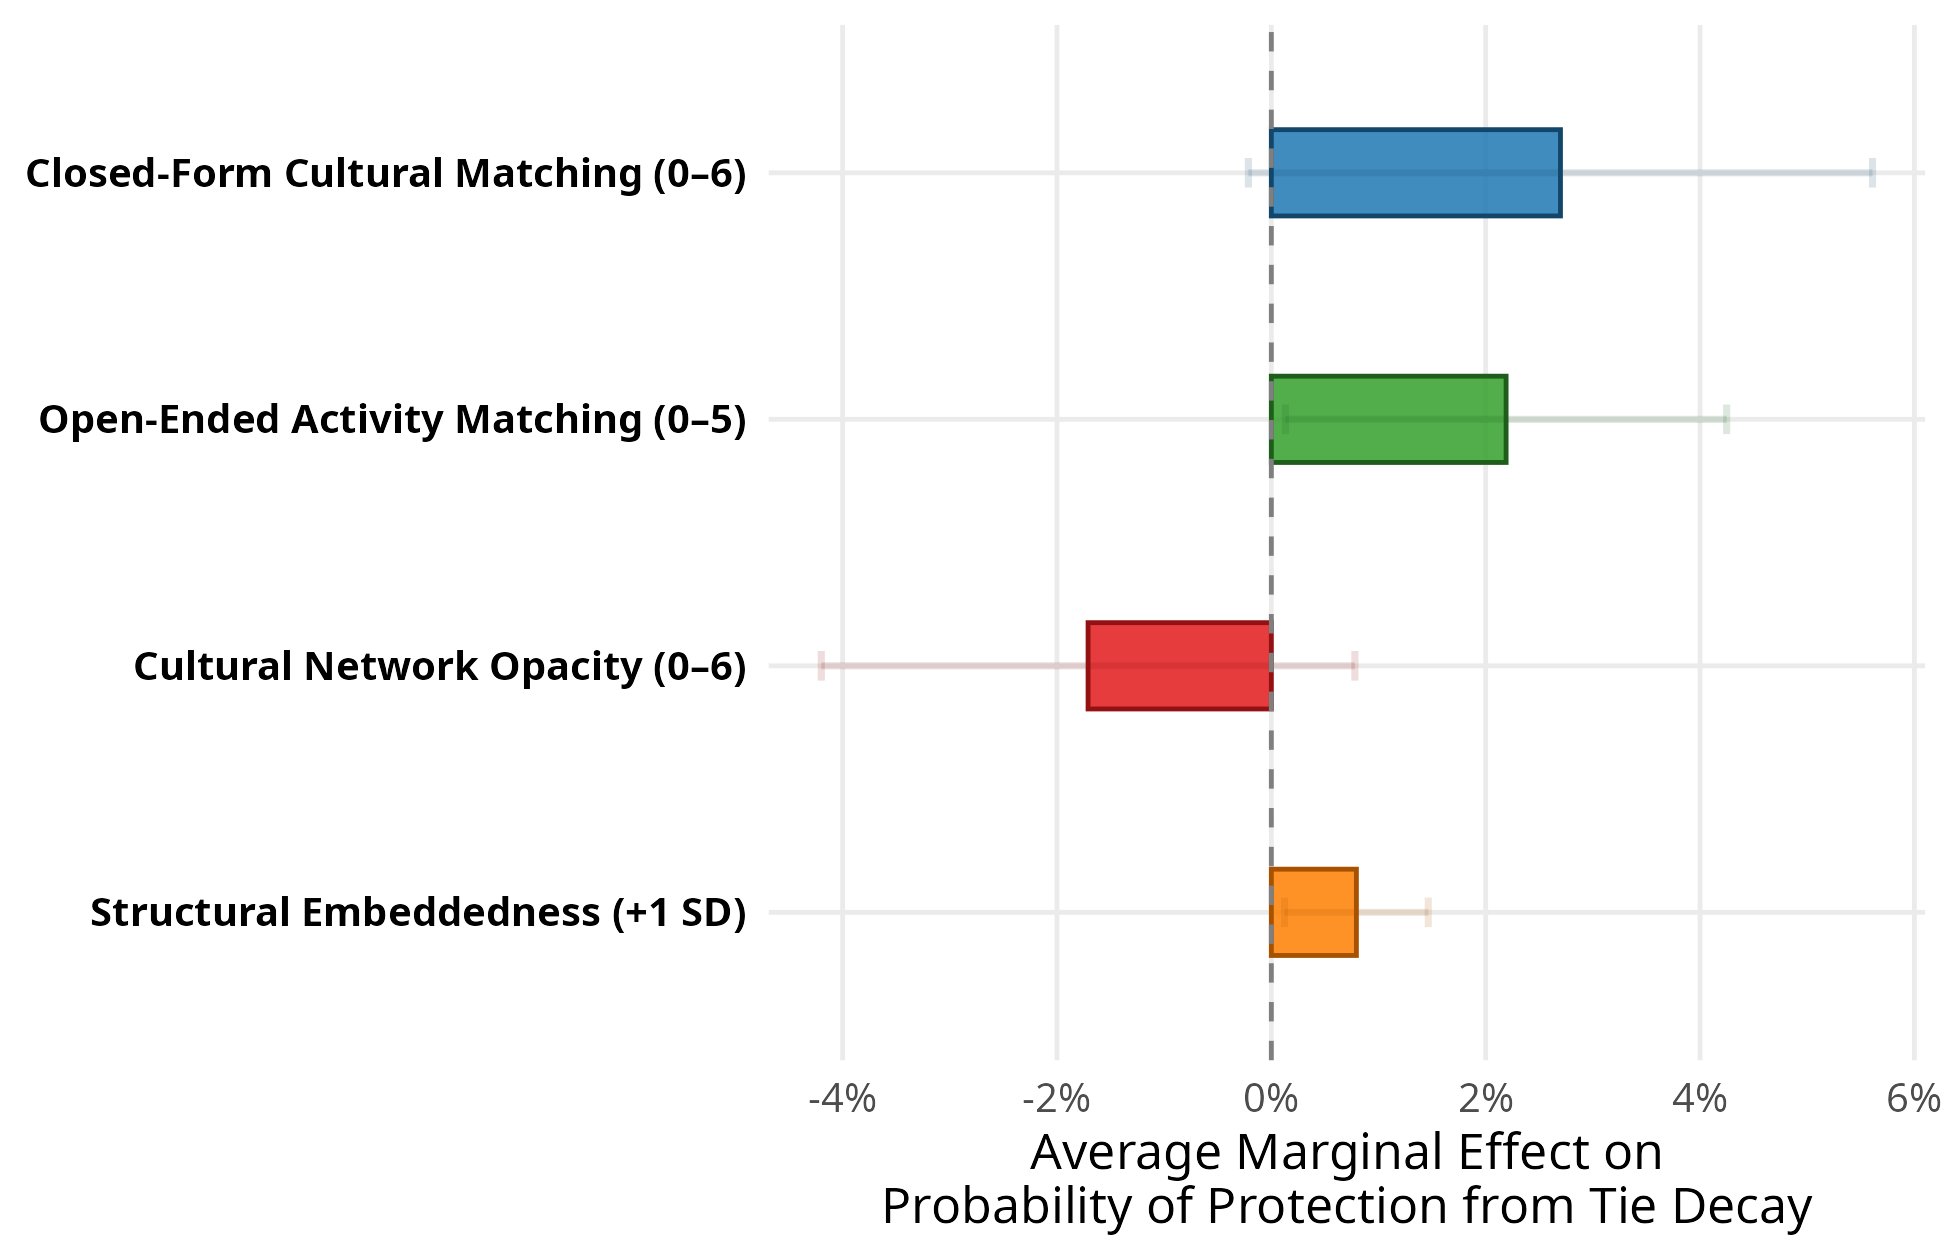
\includegraphics[width=\linewidth,keepaspectratio]{Plots/main_effects.png}
\caption{\DIFdelbeginFL \DIFdelFL{Predicted Probability of Tie Persistence by Cultural Matching and Cultural Network Opacity.}\DIFdelendFL \DIFaddbeginFL \textbf{\DIFaddFL{Predicted Probability of Protection from Tie Decay by Cultural Matching and Cultural Network Opacity.}}\DIFaddendFL }\label{fig-combined}
\end{figure}

\newpage
\begin{figure}[htbp]
\centering
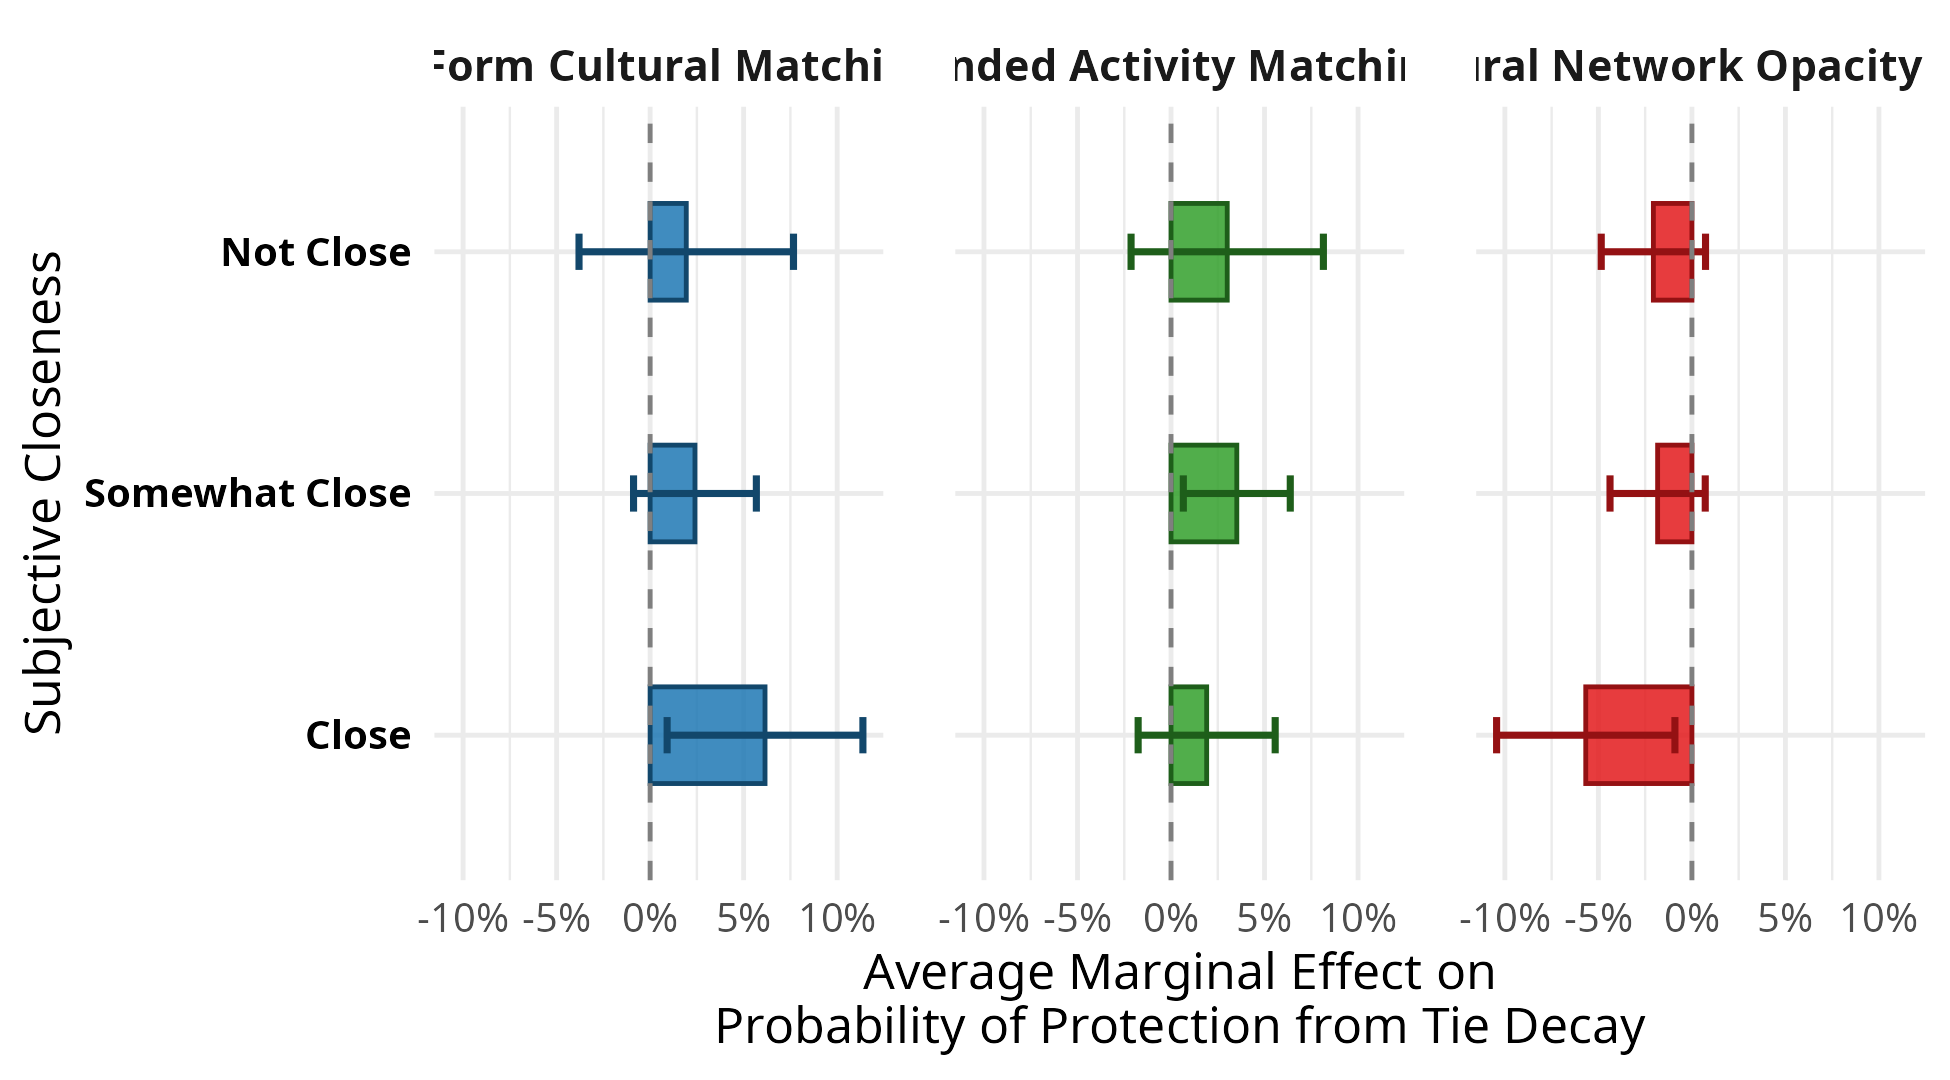
\includegraphics[width=\linewidth,keepaspectratio]{Plots/interaction_closeness.png}
\caption{\DIFdelbeginFL \DIFdelFL{Predicted Probability of Tie Persistence by Cultural Matching, Cultural Network Opacity, and Subjective Closeness.}\DIFdelendFL \DIFaddbeginFL \textbf{\DIFaddFL{Predicted Probability of Protection from Tie Decay by Cultural Matching, Network Opacity, and Subjective Closeness.}}\DIFaddendFL }\label{fig-closeness-interactions}
\end{figure}

\DIFaddbegin \newpage
\begin{figure}[htbp]
\centering
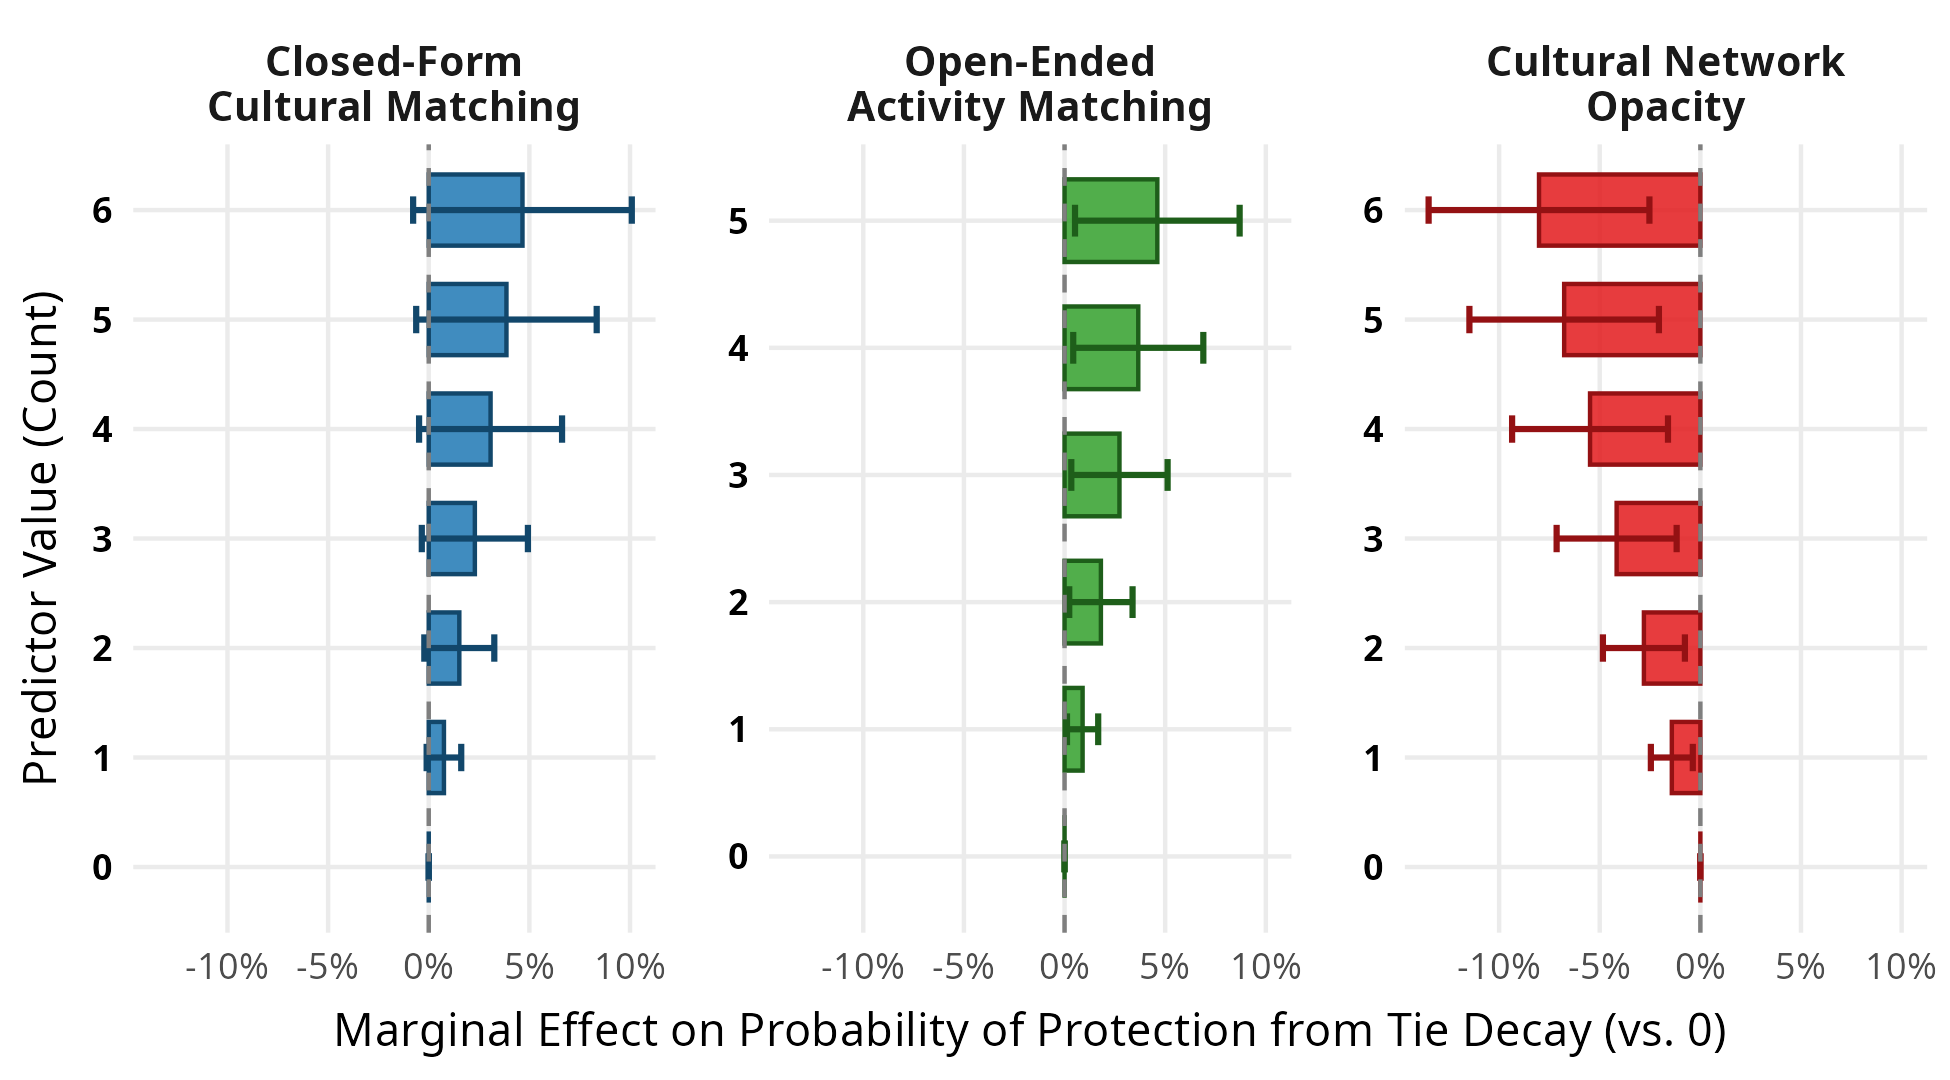
\includegraphics[width=\linewidth,keepaspectratio]{Plots/fe_predicted_probabilities.png}
\caption{\textbf{\DIFaddFL{Within-Ego Marginal Effects on Protection from Tie Decay by Cultural Matching and Opacity Counts (Ego Fixed-Effects).}}}\label{fig-fe-predictions}
\end{figure}


\DIFaddend \clearpage

\DIFdelbegin \section*{\DIFdel{References}}
%DIFAUXCMD
\DIFdelend \bibliographystyle{apalike}
\sloppy
\bibliography{manuscript_citations}

\end{document}
